
\BiChapter{基于焦点感知的光场显著性目标检测}{TODO}
\label{chap:part3}
%
%
光场显着物体检测(LFSOD)由于光场中包含丰富的空间信息而引起了广泛的关注。
与 2D (RGB) 和 3D (RGBD) 数据不同,光场本质上捕获结构化 4D 表示,包括多视图图像、深度图和焦点切片。 其中,通过眼球运动顺序观察切片的焦点堆栈,
以及迎合人类视觉感知的可见注意力转移~\cite{piao2020dut},做出适合显着性对象检测。
%
%
%
%
\BiSection{研究动机}{TODO}
%
%
%
%
%
%
一些开创性的方法~\cite{zhang2019memory,piao2020exploit}~采用 ConvLSTM~\cite{shi2015convolutional}~,它使用记忆机制以预定义的顺序单独处理焦点堆栈特征。张等人~\cite{zhang2021learning}~后来在编码器阶段采用3D卷积来提取特征。刘等人~\cite{liu2021light}~和张等人~\cite{zhang2021geometry}~使用图神经网络来聚合不同焦点切片中的上下文信息。 这些方法依赖内存使用或大量计算来提取焦点堆栈特征,从而限制了效率。
%
%
%
%
\par
%
%
%---------------------------------------------------------------------> fig: 创新图
\begin{figure}[ht]
	\centering
	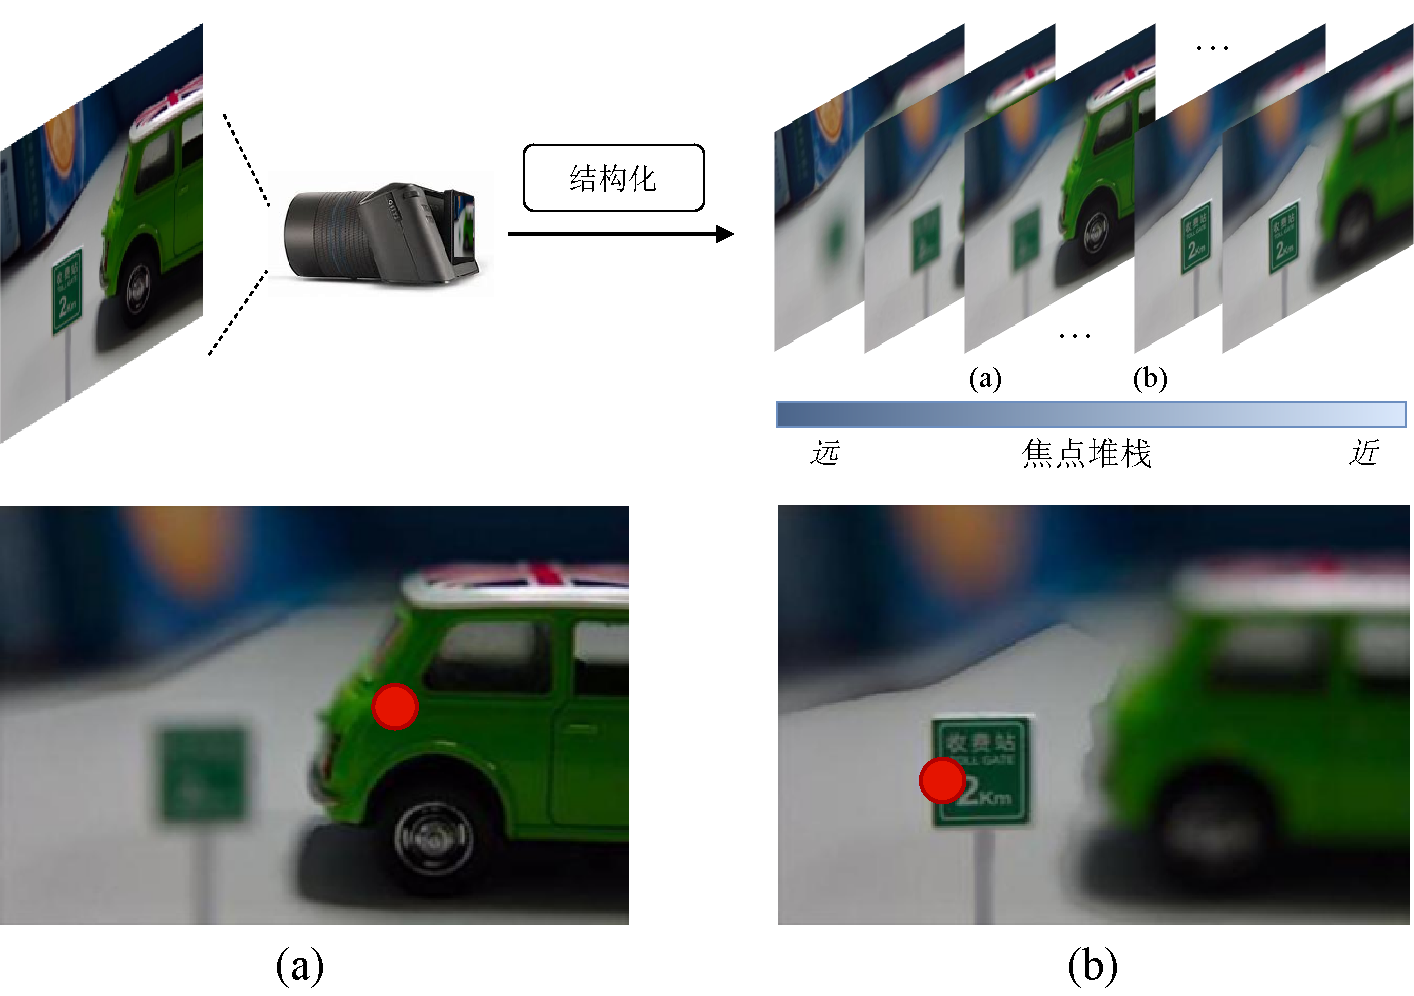
\includegraphics[width=0.85\linewidth]{figures/chapter3/cpt3_idea.pdf}
	\bicaption{%
%		光场焦点堆栈的成像原理和成像效果。
%		光场焦点堆栈的成像原理和不同切片的成像效果。
		光场焦点堆栈的成像过程和不同切片的成像效果。
%		\textbf{(a)} 远处视角包含一个清晰的汽车。
%		\textbf{(b)} 近处视角包含一个清晰的标志。
		\textcolor{red}{$\bullet$} 表示清晰的部分。
%		焦点堆栈的光场数据结构和焦点堆栈的成像效果的图示。 焦点切片具有随空间透视深度的不同而变化的聚焦部分。
%		远处的景色里有一辆清晰的汽车。
%		近景画出清晰的标志。
%		点表示透明部分。
	}
	{ %
		%			An illustration of the light field data structures to focal stack, and the imaging effect of the focal stack.
		%			% \textbf{(a)} and \textbf{(b)} indicates that 
		%			Focal slices have different sharp parts according to the distance from the lens.
		%			%%
		%			%%
		%
		%% Focal slices have different focusing parts according to the distance from the lens. 
		%
%		An illustration of light field data structures to focal stack and imaging effect of the focal stack. 
%		Focal slices have different focusing parts varying with the depth of the spatial perspective.
%		The imaging principle and imaging effect of light field focus stack.
%		The imaging principle of light field focus stack and the imaging effects of different slices.
		The imaging process of the light field focus stack and the imaging effects of different slices.
%		\textbf{(a)} The distant view contains a clear car.
%		\textbf{(b)} The close view draws a clear sign.
		\textcolor{red}{$\bullet$} indicates the clear parts.  
	}
	\label{figure:cpt3:idea}
	
	%				 		\vspace{-0.25cm}
\end{figure}
%
%
%
%
我们重新思考光场数据建模的方式。考虑到焦点堆栈的成像效果,如图~\ref{figure:cpt3:idea}~所示,每个焦点切片根据空间透视深度的不同,聚焦部位也不同。 并且从同一场景生成,焦点切片有很多共同点。
因此,即使在很小的带宽内,也可以充分总结和传达它们之间的差异。 此外,给定图像,人类可以毫不费力地关注敏感部分并忽略不重要的背景。 因此,在焦点堆栈中处理更多相对的焦点切片来模拟人类视觉系统是合理的。 
%
%
%
%
\par
%
%

受上述观察的启发,我们考虑两个关键问题:
%
%
%
%
1)我们如何设计一个模型来存储切片级特征并在焦点堆栈和全焦点图像之间传递信息以进行上下文建模? 
2)我们如何设计一个模型来理解场景的空间分布并感知敏感的焦点切片? 
%
%
%
%
\par
在本文中,我们提出了一种用于高效且有效的 LFSOD 的焦点感知Transformer(FPT)。 具体来说,我们收集图像特定的特征并制定通信以加强焦点堆栈和全焦点图像之间的相互感知。 我们利用选择性机制将适当的焦点切片纳入检测。 具体来说,我们的贡献有三个:
%
%
%
%
\par
%
%
%
%
\begin{itemize}
	\item 我们引入与焦点相关的标记来总结图像特定的特征,并提出一种标记通信模块(TCM),通过计算与焦点相关的标记之间的交叉注意力来执行特征交互。 我们转移焦点堆栈中与焦点相关的标记以促进空间上下文传播。 
	
	\item 我们提出了一种焦点感知增强(FPE)策略,通过切片选择机制来增强焦点堆栈中的特征空间表示,以有区别地处理适当的焦点切片。	这可以突出显着切片并抑制非显着区域的干扰。 
	
	\item 我们对 4 个广泛使用的数据集进行了广泛的实验,并证明我们的方法优于现有最先进的 LFSOD 方法。 我们的方法在 DUTLF-FS~\cite{zhang2019memory}~上将 MAE 指标显着降低了 31\%。
\end{itemize}


 RBG显著性目标检测(SOD)~\cite{ ma2021pyramidal, wei2020f3net, zhou2020interactive}~、
 RGB-D~\cite{ cong2022cir, ji2021calibrated, liu2021visual}~和光场图像一直是活跃的研究领域。 
 在本文中,我们将主要研究LFSOD任务。
 现有的光场显着目标检测方法大致可以分为两类:(1)传统方法;(2)基于深度学习的方法。 传统方法通常采用手工制作的特征(例如,颜色对比度、纹理对比度和深度对比度)和先验(例如,位置先验、背景先验和边界连接先验)来检测显着对象。 
% 
%
%
%
 李等人~\cite{li2014saliency}~提出了第一个光场显着性数据集,并通过计算背景先验、位置先验和对比度线索来检测显着对象。
 之后,李等人~\cite{li2015weighted}~提出了加权稀疏编码框架同时处理2D、3D和4D SOD问题。
 张等人~\cite{zhang2015saliency}~计算对比度显着图,然后使用背景先验来消除背景干扰并获得最终结果。 
 张等人~\cite{zhang2017saliency}~基于随机搜索策略集成了从全焦点图像、深度图、焦点切片和多视图图像中提取的多个光场线索。 
 最近,Piao 等人~\cite{piao2019saliency}~提出了 LFSOD 的深度诱导元胞自动机。
 有关传统方法的更多详细信息可以在\cite{fu2022light}~中找到。
 到了深度学习时代,几种深度学习方法对光场SOD性能有了显着提升。 
 朴等人~\cite{piao2019deep}~首次尝试引入CNN来提取光场语义特征,并获得相应的显着图。 
 王等人~\cite{wang2019deep}~应用ConvLSTM~\cite{shi2015convolutional}~来融合CNN生成的特征,然后预测显着图。
 张等人~\cite{zhang2019memory}~还利用ConvLSTM来利用光场,并提出了用于显着性检测的最大光场数据集。 
 张等人~\cite{zhang2020lfnet}~利用提出的细化模块和集成模块的集成焦点堆栈特征来开发焦点切片。
朴等人~\cite{piao2020exploit}~提出了一种由焦点流和RGB流组成的不对称双流架构,以实现台式计算机和移动设备的多功能性。
%
%
%
%
\par
%
尽管大多数方法输入全焦点图像和焦点堆栈,但一些方法\cite{jing2021occlusion, wang2022lfbcnet, zhang2022exploring}~提出使用多视图和中心视图图像来检测显着对象。 
张等人~\cite{zhang2020light}~提出了一种深度网络,通过利用微透镜图像中丰富的角度信息来检测显着物体。 
张等人~\cite{zhang2021geometry}~提出了一种图神经网络,通过有效探索多视图图像之间的空间和视差相关性来预测显着图。 
静等人~\cite{jing2021occlusion}~提出了一种遮挡感知网络,从极平面图像(EPI)中提取遮挡边界特征以进行显着性检测。 
张等人~\cite{zhang2022exploring}~提出了一种光场合成网络来产生可靠的4D信息并驱动显着性检测。 
然而,上述方法的性能不如基于焦点堆栈输入的常见方法。 

这些使用焦点堆栈作为输入的方法集成了解码器中整个焦点堆栈的特征,忽略了不同切片对检测的相对贡献,并且容易受到非显着背景的影响。 因此,我们提出了更为适合 LFSOD 任务的设计。
 

Transformer,首先由 Vaswani 等人提出~\cite{vaswani2017attention}~,已广泛应用于自然语言处理(NLP)。
ViT 由 Dosovitskiy 等人提出~\cite{dosovitskiy2020image}~,首先将Transformer应用于图像域。 由于其强大的全局信息捕获能力,Transformer表现出了优异的性能。
最近的工作探索了将 Transformer 应用于各种视觉任务:
图像分类~\cite{chen2020generative, dosovitskiy2020image}~、
对象检测~\cite{zhu2020deformable, dai2021up, sun2021rethinking}~、
分割~\cite{chen2021pre, wang2021end}~、
图像增强~\cite{yang2020learning, chen2021pre}~、
图像生成~\cite{parmar2018image}~和 
视频处理~\cite{zhou2018end, zheng2020end}~,
以缓解 CNN 有限的全局信息学习能力。 此外,Transformer 已广泛应用于 RGB 显着目标检测~\cite{liu2021visual, siris2021scene}~和 RGBD 显着目标检测~\cite{liu2021tritransnet, wang2021mutualformer}~,例如,
刘等人~\cite{liu2021visual}~设计了一个基于纯Transformer架构的统一模型,通过建模远程依赖性来预测显着性。 
刘等人~\cite{liu2021tritransnet}~提出了一种用于 RGB-D 显着目标检测的三元组变换器嵌入模块,通过学习跨层的远程依赖关系来增强高级特征。 
塞里斯等人~\cite{siris2021scene}~提出了一种上下文实例转换器来捕获对象和场景上下文之间的上下文关系,以实现更准确的显着性推断。 
王等人~\cite{wang2021mutualformer}~提出了一种基于Transformer的多模态融合模块来增强和融合RGB和深度图像特征。
受益于Transformer的使用,这些方法可以获得更准确的场景上下文特征,并在复杂场景中表现出更好的检测性能。 然而,如何将Transformer应用于 LFSOD 尚未得到全面探讨。 考虑Transformer在建立长期依赖方面的优势,适合总结图像特定特征并通过附加标记传达信息。 在本文中,我们提出了一种令牌通信模块(Token Communication
Module,TCM)来加强信息交互并促进上下文特征感知。
%
%
%
%
\BiSection{方法介绍}{TODO}
%
%
%
%
%\par
\begin{figure}[!ht]
	\centering
	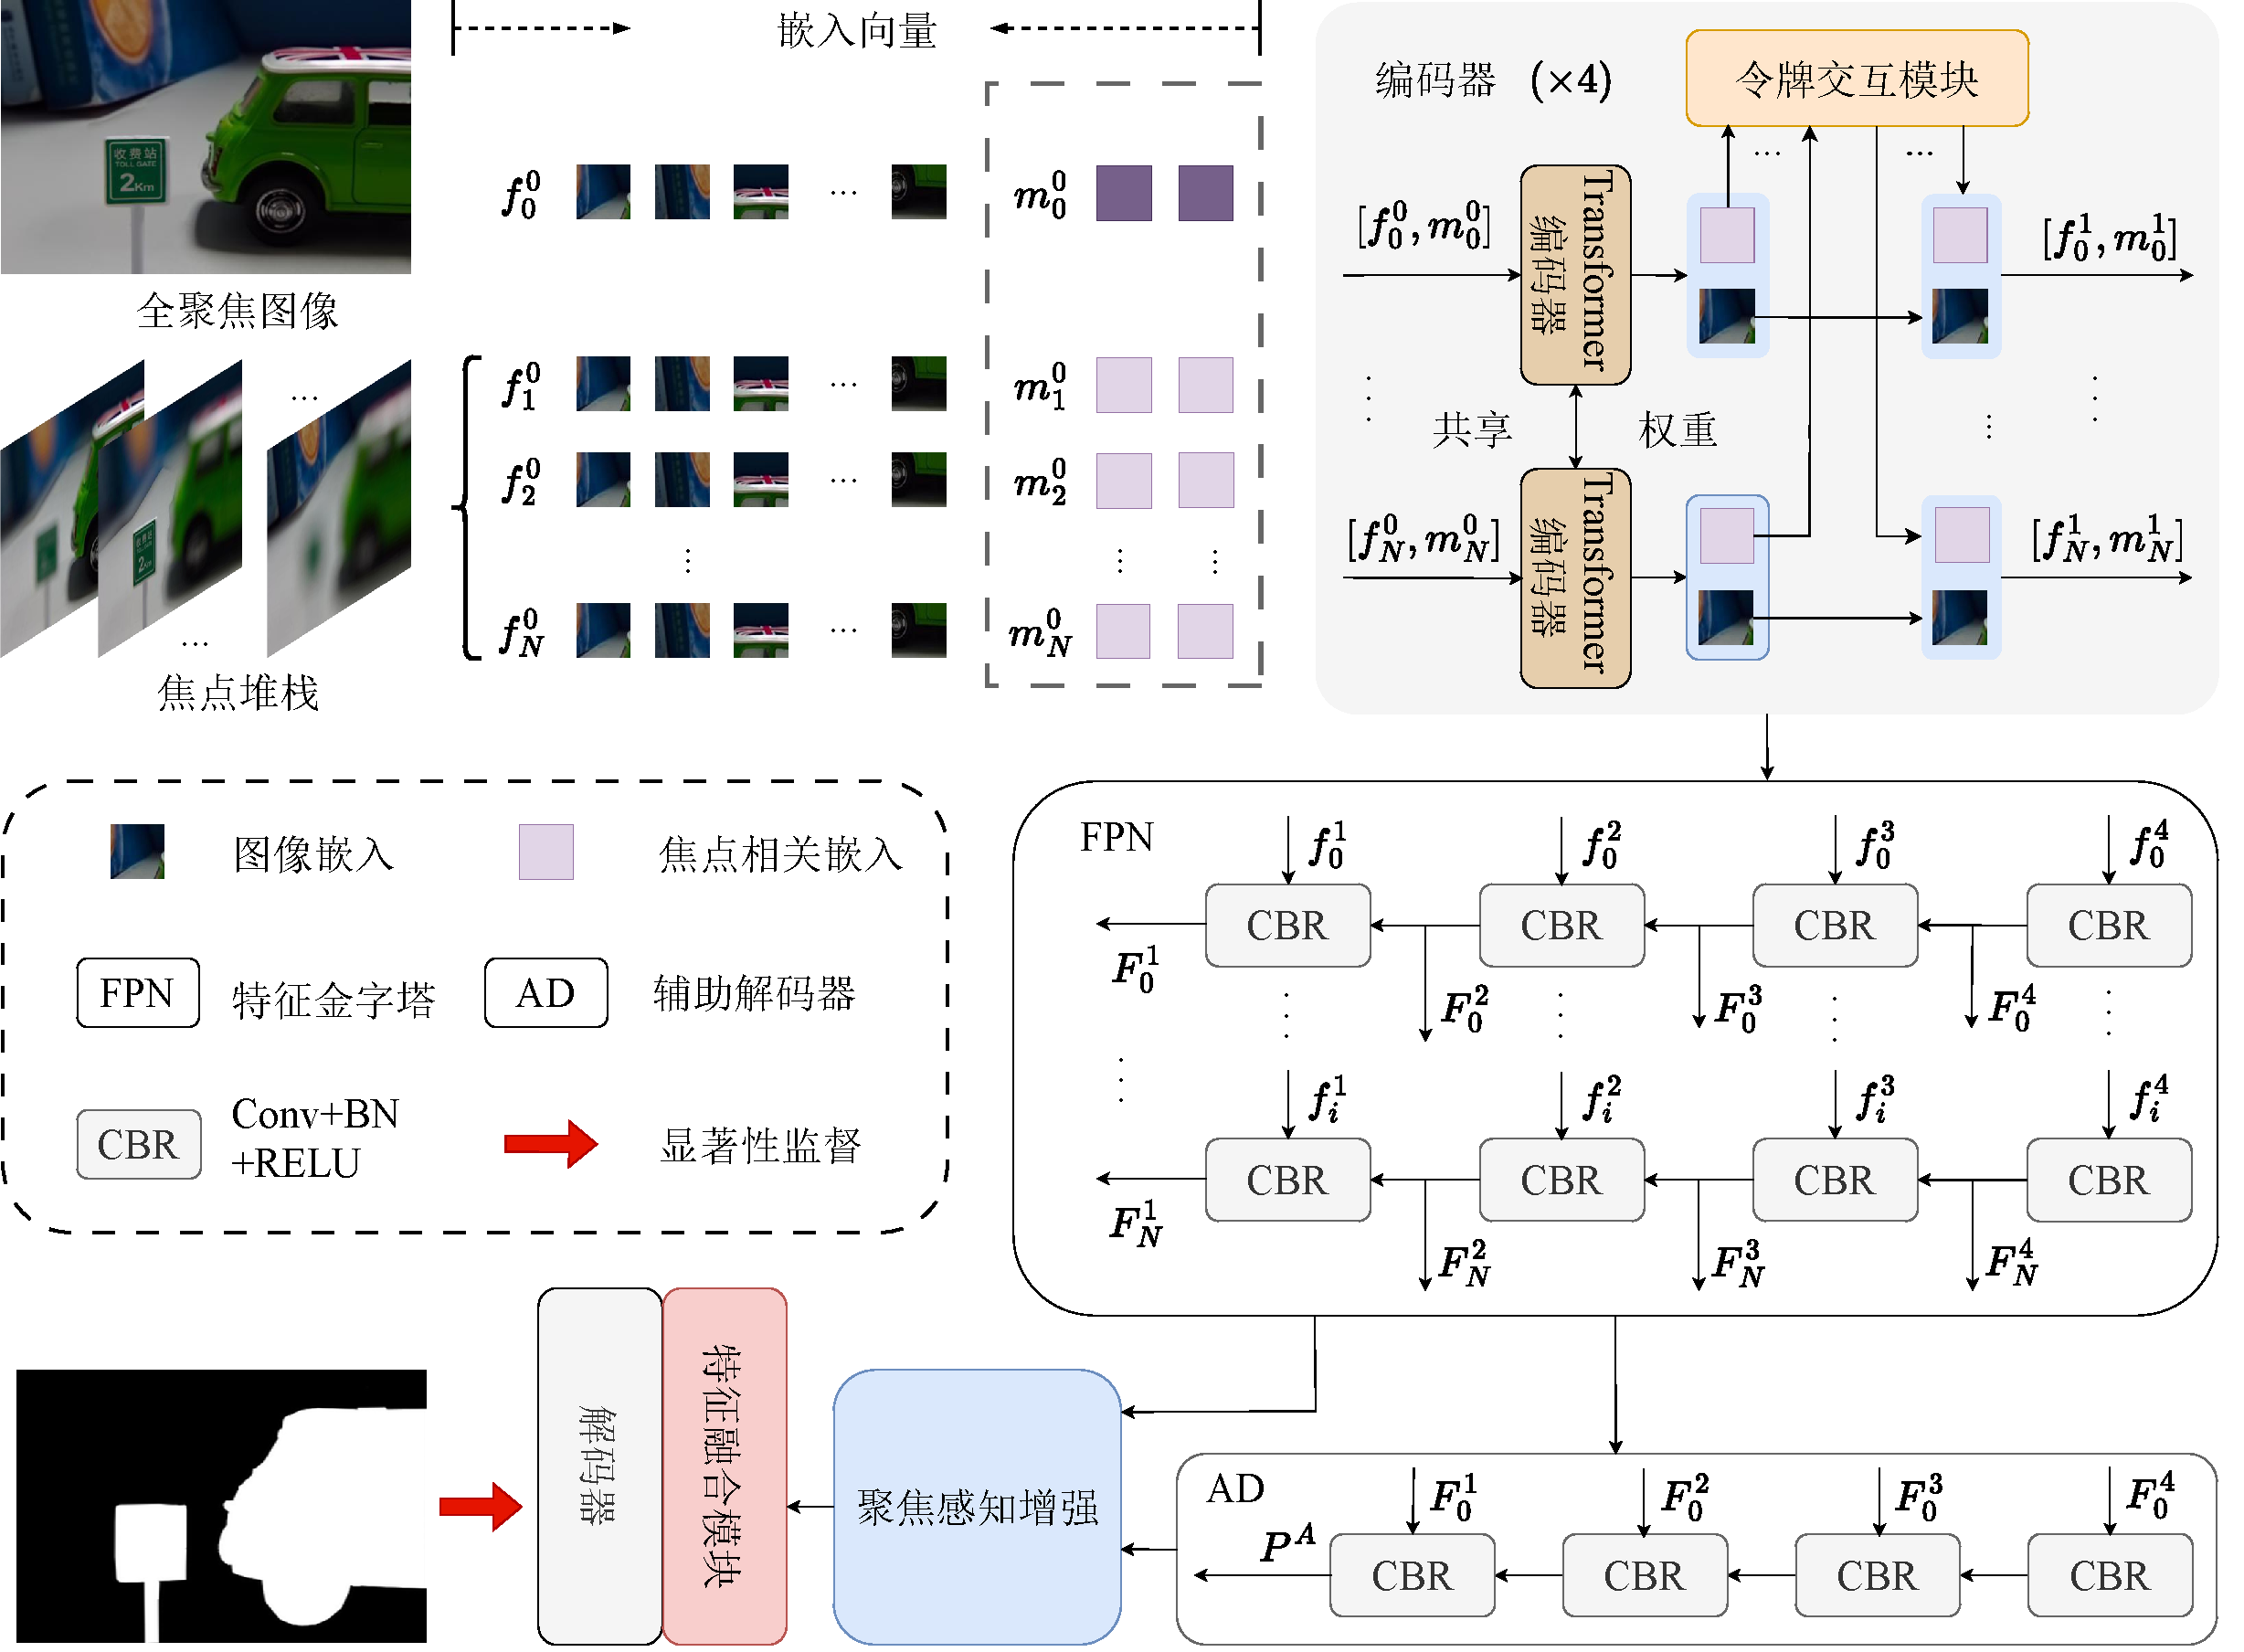
\includegraphics[width=0.95\linewidth]{figures/chapter3/overview_1}
	\bicaption{
%		整体网络结构图。
		光场显著性目标检测网络的架构。
	}{
		The architecture of light field salient object detection network.
	}  
	\label{cpt3_fig1:overview}
\end{figure}
%
%
%
%
%
我们提出的 FPT 的整体架构如图 2 所示。给定 $N + 1$ 个分辨率为 $ H \times W $ 的图像,包括一个全焦点图像和 $N$ 个焦点堆栈图像,我们将每个图像划分为补丁区块作为输入。 
将展平的 $N$ 个 patch 输入到线性投影中,得到嵌入的 patch $ \left \{ f_{i}^{0} \right \}_{i=0}^{N} $,其形状为$ \left ( N + 1 \right ) \times \frac{HW}{P^{2}} \times C  $,其中 $P$ 表示每个 patch 的大小,$C$ 表示每个 patch 的大小。 
渠道维度。 
%
%
%
具体地,$ f_{0}^{0} $ 表示全焦点图像的特征输入。 
$ \left \{ f_{i}^{0} \right \}_{i=1}^{N} $ 表示焦点堆栈的特征输入。 
此外,为了总结补丁中的信息,引入了一组大小为 $ M \times C $ 的随机初始化的可学习嵌入,作为 { }N 个焦点相关标记,表示为 $ \left \{ m_{i}^{0} \right \}_{i=0}^{N} $ ,其中 $M$ 表示焦点相关标记的数量。 
我们将每个 patch 与焦点相关的标记连接起来,
并得到 $ \left \{ \left [ f_{i}^{0},m_{i}^{0}  \right ]  \right \}_{i=0}^{N} $ 作为特征提取器的输入。 
%
%
%
%
%
\par
%
%
与卷积网络使用不同的卷积步长来获得多尺度特征图不同,
我们使用渐进收缩策略通过patch嵌入层来控制特征图的尺度。
我们用$ l \in 1..T $ 表示阶段编号。 
我们将第$l$个阶段补丁块大小表示为$P_{l}$,在第$l$阶段开始时,
我们首先均匀划分输入特征图
$F_{l-1} \in \mathbb{R}^{H_{l-1} \times W_{l-1} \times C_{l-1}}$
为
$ \frac{H_{l-1}W_{l-1}}{P_{l}^{2}} $
个补丁块。

然后,将每个补丁块展平并投影到$C_{l}$维度的嵌入表达。
在线性投影之后,嵌入补丁的形状可以看做是
$\frac{H_{l-1}}{P_{l}} \times \frac{W_{l-1}}{P_{l}} \times C_{l} $,
其中高度和宽度比输入小了$P_{l}$倍。
这样我们可以灵活调整每个阶段的特征图的尺度,
使得可以构建基于Transformer的特征金字塔。
%
%
%
%
第$l$阶段的Transformer编码器有 $ N_{i} \in [3,4,6,3] $ 个 Transformer 块。
%
%
%
%
%
%\par
\begin{figure}[!ht]
	\centering
	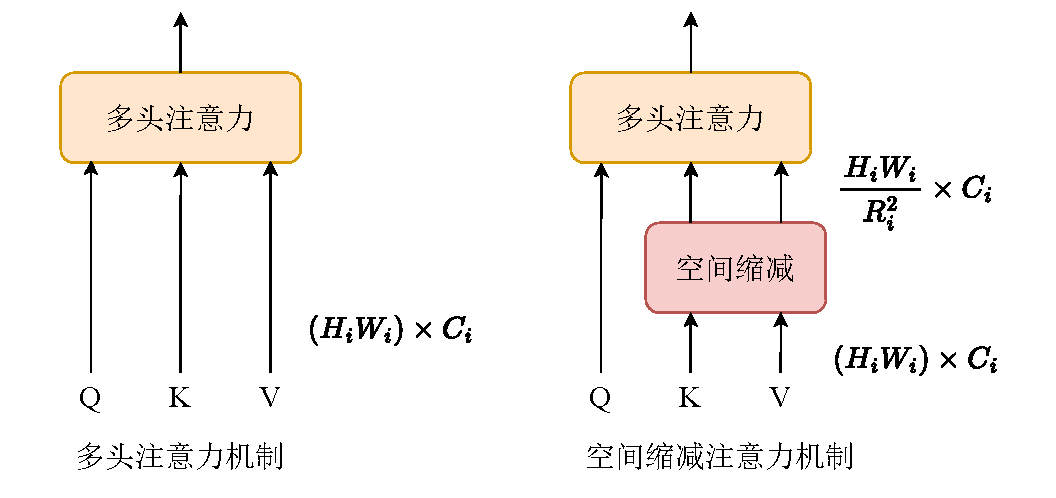
\includegraphics[width=0.95\linewidth]{figures/chapter3/sra}
	\bicaption{
		令牌通信模块 (TCM) 的图示。
		(a) 令牌交互(TI)。 
		%		交叉注意力在全焦点和焦点堆栈的嵌入式令牌之间执行特征交互。 
		(b) 令牌移位(TS)。 
		%		仅将焦点堆栈流中与焦点相关的标记分成组(图中以2组为例),然后沿焦点深度轴以不同方向(左右)移位以交换切片级信息。
	}{
		An illustration of the Token Communication Module (TCM). 
		(a) Token Interaction (TI). 
		%	Cross-attention performs feature interactions between the all-focal and focal stack. 
		(b) Token Shift (TS).
		%	Only the focus-related tokens in the focus stack stream are split into groups (2 in the figure) and then circularly shifted along the focus-depth axis with different directions to exchange slice-level information.
	}  
	\label{cpt3_fig1:sra}
\end{figure}
%
%
%
%
%
\par
%
%
我们构造基于金字塔Transformer(Pyramid Vision Transformer,PVT)~\cite{wang2022pvt}~的主干网由 $T = 4$ 个阶段组成。 
%
%~
%
由于骨干网络需要处理高分辨率的特征图,我们采用空间缩减注意力(Spatial-Reduction Attention,SRA)来取代Transformer编码器~\cite{vaswani2017attention}~中传统多头注意力(Multi-Head Attention)层。
%
%\\
%
%\\
%
\par 
%
%
与多头注意力机制类似,空间缩减注意力接受查询$Q$、秘钥$K$和值$V$作为输入,并细化输出的特征。
不同之处在于,仅需注意力操作之前缩减了$K$和$V$的空间尺度,如图~\ref{cpt3_fig1:sra},
能够在很大程度上减少计算和内存开销。
第$l$阶段的空间缩减注意细节可以表述如下:
%
%
%
%
\begin{equation}
	SRA(Q,~K,~V) = Concat(head_{0},~ \cdots,~ head_{H_{l}})~W^{O}
\end{equation}
%
%
\begin{equation}
	head_{j} = Attention(Q~W_{j}^{Q}, ~ SR(K)~W_{j}^{K},~ SR(V)~W_{j}^{V})
\end{equation}
%
%
%
其中$Concat(\cdot)$是连接操作。
$W_{j}^{Q} \in \mathbb{R}^{C_{i} \times d_{head}},~
W_{j}^{K} \in \mathbb{R}^{C_{i} \times d_{head}},~
W_{j}^{V} \in \mathbb{R}^{C_{i} \times d_{head}},~$
和
$W^{O} \in \mathbb{R}^{C_{i} \times C_{i}}~$
是线性映射参数。
$H_{l}$是每个阶段注意力层的头数。
$SR(\cdot)$是减少输入序列空间维度的操作,它的公式是:
%
%
%\\
%
\begin{equation}
	SR(x) = Norm(Reshape(x, R_{l})W^{S})
\end{equation}
%
%
其中$x \in \mathbb{R}^{(H_{l}W_{l}) \times C_{l}} $
表示输入序列,$R_{l}$表示每个阶段中的注意力层的缩减比例。
$Reshape(x, R_{l})$ 表示将输入序列 $x$ 重塑大小为
$\frac{H_{l}W_{l}}{R_{i}^{2}} \times (R_{i}^{2}C_{i})$。
$W_{S} \in \mathbb{R}^{R_{i}^{2}C_{i}}$
是一个线性投影,它将输入序列的维度减少到$C_{l}$。
$Norm(\cdot)$指的是层归一化。
%
%
\par
%
%
与原始的Transformer~\cite{vaswani2017attention}~中一样,
我们的每个 Transformer 块包括线性空间减少注意力 (SRA) 和前馈网络 (FFN),
以每个图像的方式作用于联合注意学习:
%%
%%
\begin{equation}
	\left \{ [f_{i}^{l}, m_{i}^{l}]\right \}_{i=0}^{N} = \left \{ FFN^{l} \left  ( SRA^{l} \left ( [f_{i}^{l-1}, m_{i}^{l-1}]\right )\right )\right \}_{i=0}^{N},
\end{equation}
%%
%%
每个Transformer编码器后面都布置了令牌通信模块(TCM),用于特征通信。 
%
%
%
%
%
%
%
%
%
%
%
%
%
%
\par
经过特征提取,我们从 Transformer 块的输出中得到四层特征 
$\left \{ f_{i}^{1},f_{i}^{2},f_{i}^{3},f_{i}^{4} \right \}_{i=0}^{N}$ 。 
之后,采用共享权重特征金字塔网络(FPN)~\cite{lin2017feature}~进行分层融合并得到 $N$ 个金字塔特征图	$ \left \{F_{i}^{1},F_{i}^{2},F_{i}^{3},F_{i}^{4} \right \}_{i=0}^{N}$:
%%
%%
\begin{equation}
	\begin{aligned}
		F_{i}^{4} &= Up \left ( CBR \left ( f_{i}^{4} \right )\right ) \\ 
		F_{i}^{l} &= Up \left ( CBR \left ( f_{i}^{l} + F_{i}^{l+1} \right )  \right ),l=1,2,3  .
	\end{aligned}
\end{equation}
%%
%%
其中 $Up$ 贡献 $2 \times $ 上采样 操作时,$CBR$ 表示一个卷积块,包括 Conv+ BN+ RELU 层。 对于解码器,提出的焦点感知增强(FPE)策略增强了焦点堆栈的特征表示。 增强的焦点堆栈和全焦点特征融合在特征融合模块(FFM)中。 最后,采用掩模解码器来生成显着图。
%
%
%
%
%
\BiSubsection{令牌交互模块}{TODO}
%
%
%
%
%
%\par
\begin{figure}[!ht]
	\centering
	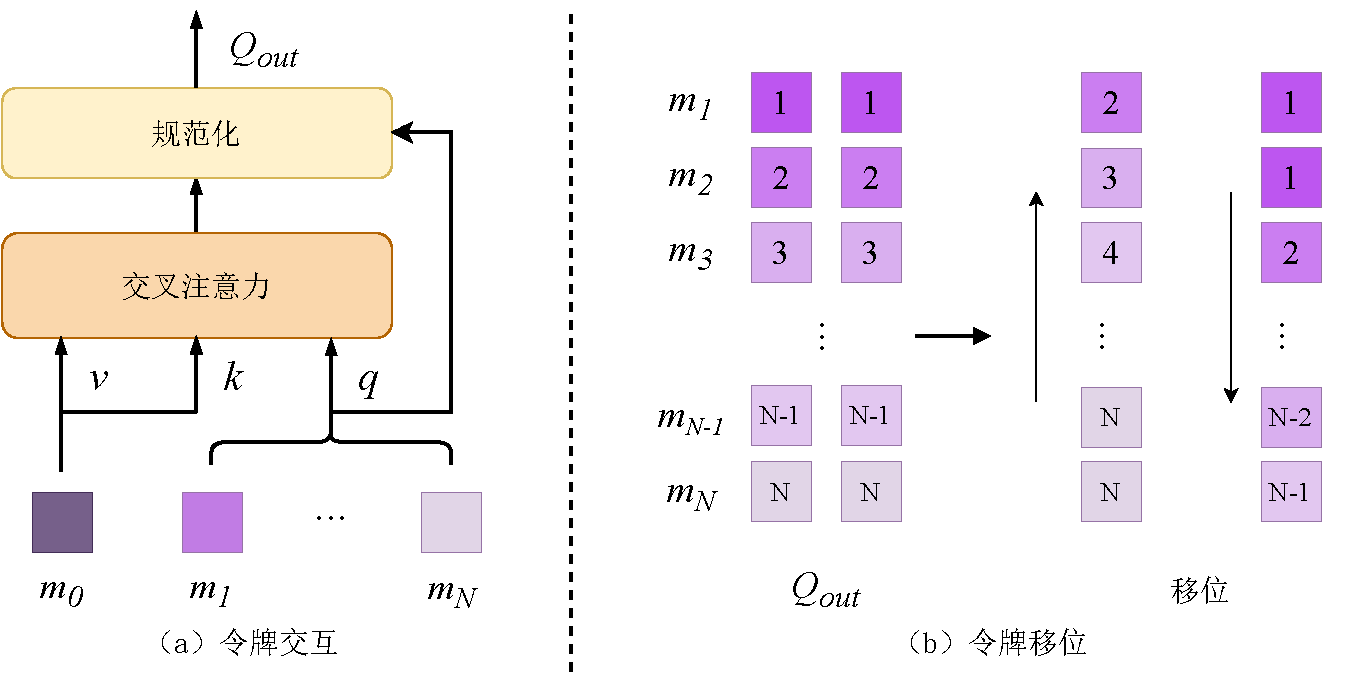
\includegraphics[width=0.95\linewidth]{figures/chapter3/token-interaction.drawio}
	\bicaption{
		令牌通信模块 (TCM) 的图示。
		(a) 令牌交互(TI)。 
%		交叉注意力在全焦点和焦点堆栈的嵌入式令牌之间执行特征交互。 
		(b) 令牌移位(TS)。 
%		仅将焦点堆栈流中与焦点相关的标记分成组(图中以2组为例),然后沿焦点深度轴以不同方向(左右)移位以交换切片级信息。
	}{
	An illustration of the Token Communication Module (TCM). 
	(a) Token Interaction (TI). 
%	Cross-attention performs feature interactions between the all-focal and focal stack. 
	(b) Token Shift (TS).
%	Only the focus-related tokens in the focus stack stream are split into groups (2 in the figure) and then circularly shifted along the focus-depth axis with different directions to exchange slice-level information.
	}  
	\label{cpt3_fig1:token_interaction}
\end{figure}
%
%
%
%
在以前的光场显著性检测方法中,主干网络仅以原像方式执行特征提取~\cite{piao2020exploit, liu2021light},忽略了光场数据固有的丰富上下文信息。 相比之下,我们设计了一个令牌通信模块(Token Communication Module,TCM)来对全焦点和焦点堆栈进行上下文建模,如图~\ref{cpt3_fig1:token_interaction}~所示。
TCM 由令牌交互(Token Interaction,TI)和令牌移位(Token Shift,TS)操作组成。 
令牌交互模块在全焦点和焦点堆栈的焦点相关令牌之间进行交叉注意力计算,以进行信息交互。 
令牌移位操作通过转移焦点堆栈中与焦点相关的标记,以促进上下文特征感知。 
%
%
%
%
%
\par
\textbf{令牌交互:}
如图~\ref{cpt3_fig1:token_interaction}~(a)~所示,令牌交互由交叉注意力 (Cross Attention,CA) 块组成。 
注意力函数可以描述为将查询和一组键值对映射到计算为值的加权和的输出。 
分配给每个值的权重是查询与相应键之间的相似度。 
这里,我们采用带有残差连接和层归一化的缩放点积注意力来实现交叉注意力块,公式可以表述如下:
%\todo
%
%
%
%%
\begin{equation}
	Attention(Q,K,V) = softmax \left ( \frac{QK^{T}}{\sqrt{d_{k}}} \right ) V,
\end{equation}
%%
%%
%
%
其中
$ Q \in \mathbb{R}^{N_{q}\times d_{k}}  $,
$ K \in \mathbb{R}^{N_{k}\times d_{k}}  $ 和
$ V \in \mathbb{R}^{N_{v}\times d_{k}}  $ 
分别是查询、键和值。 
$ d_{k} $ 是查询和密钥的通道维度,
$ \sqrt{d_{k}} $ 是控制softmax分布的温度参数。 
对于交叉注意力块,$K$ 和 $V$ 是相同的。 
%
%
%
%
%
\par
%
%
%
%
交叉注意力块将所有与焦点相关的标记 $ \left \{ m_{i}^{l} \right \}_{i=0}^{N} $ 作为输入。 焦点堆栈流的标记 $ \left \{  m_{i}^{l} \right \}_{i=1}^{N} $ 用作查询来计算与属于全焦点流的键 $ m_{0}^{l} $ 的相似度并从值 $ m_{0}^{l} $ 检索焦点信息。 该交叉注意力块的输出 $ Q_{out}^{l} $ 可计算如下:
%
%
%%
%%
\begin{equation}
	Q_{out}^{1} = LN \left ( Attention(Q,K,V) + Q \right ),
\end{equation}
%%
%%
%
%
其中
$ Q = \left \{ m_{i}^{1} \right \}_{i=1}^{N}~ W^{Q}$,
$ K= m_{0}^{1} ~W^{K} $,
$ V =  m_{0}^{1}~ W^{V} $。
$ Q$,$K$,$V$ 和 $ Q_{out}^{l} $
的维度分别为 
$ N \times M \times C $,$ M \times C $,$ M \times C $ 
和
 $ N \times M \times C $。 
%
%
%\\
%
\par
%
%
%
\textbf{令牌移位:}
%
%
上述操作的输出 $ Q_{out}^{l} $ 被馈送到令牌移位操作中,
如图~\ref{cpt3_fig1:token_interaction}~(b)~中所示。 
与焦点相关的标记被分为 $G = 2$ 组,并沿着焦点深度轴以不同方向(向前或向后)移动。 
对于每组焦点相关嵌入表示,可以看做是整体往左(或右)移动了一个图像级切片的位置。
经过一次移位操作,
每一张切片所对应的焦点相关嵌入由其左右两张切片的焦点相关嵌入的共同组合,
而对于两端的散焦切片,只汇总了一个方向上的不同图片的焦点相关嵌入信息。
%
%
%
%\\
%
%
\par
%
%
通过不同的焦点深度和方向,令牌可以实现与近深度和远深度焦点图像的空间特征进行上下文交换。 
然后我们用连接的 $ \left \{ m_{i}^{l} \right \}_{i=0}^{N} $ 更新所有与焦点相关的标记  $ \left \{ m_{i}^{l} \right \}_{i=0}^{N} $ 并将 
$ Q_{out}^{l} $ 移出。 
%
%
%\\
%
%
%\par
%
%
这种设计的目的是随着网络的深入,能够促进网络对于光场三维场景的整体感知,
从而保持稳定的空间感受野。 
值得一提的是,令牌移位操作几乎是无参数的,带来的计算成本可以忽略不计。


\BiSubsection{聚焦感知增强策略}{TODO}
%
%
%
%
受人类视觉注意系统中关注选择性的启发,我们的目标是从多焦点特征中有效地感知有用的显着性信息。 我们提出了一种焦点感知增强(Focus Perception Enhancement,FPE)策略来模仿人类如何从视觉资源中选择感兴趣信息的筛选阶段。 
聚焦感知增强模块由切片选择机制组成,
用于有区别地处理焦点相关切片,
如图~\ref{cpt3_fig1:fpe}~所示。
选择机制可以突出显着切片并抑制非显着区域的干扰。 
此外,我们采用结构相似性~\cite{wang2003multiscale}~来评估焦点切片和全焦点图像之间焦点的一致性,
因为散焦状态下的物体不具有清晰的纹理结构。 
%
%
%
%
%\par
\begin{figure}[!ht]
	\centering
	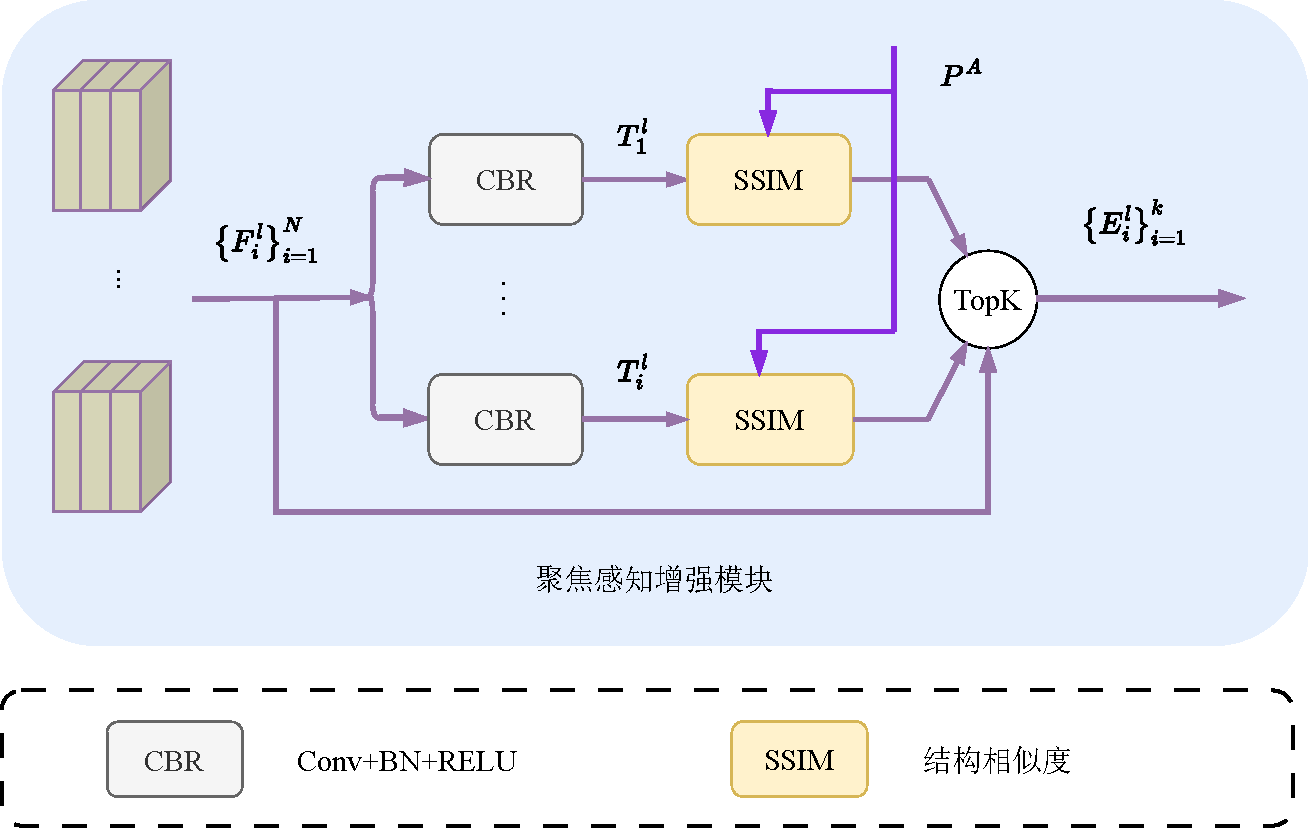
\includegraphics[width=0.90\linewidth]{figures/chapter3/fpe}
	\bicaption{
		聚焦感知增强模块。
	}{
		Focused perception enhancement module.
	}  
	\label{cpt3_fig1:fpe}
\end{figure}
%
%
%
%
\par
%
%
首先,我们使用基于特征金字塔网络的辅助解码器(Auxiliary Decoder,AD)生成辅助显着性预测 $ P^{A} $ 并应用监督以避免非显着对象的干扰并确保全焦点特征的有效性。 然后,我们使用全焦点显着性预测 $ P^{A} $ 计算焦点堆栈 $ \left \{ F_{i}^{l} \right \}_{i=1}^{N} $ 的每个层特征的结构相似度得分。 
%%
%%
\begin{equation}
	score_{i}^{l} = SSIM \left ( CBR \left ( F_{i}^{l} \right ), P^{A} \right ),
\end{equation}
%%
%%
%
%
其中 $CBR$ 表示一个卷积块,它将特征通道压缩成一维。 $SSIM$ 表示结构相似度,可以表示为: 
%
%
%%
%%
\begin{equation} 	
	SSIM(x,y)=\frac{\left ( 2\mu_{x}\mu_{y}+C_{1} \right ) \left (  2\sigma_{xy}+C_{2} \right )  } 	
	{\left ( \mu_{x}^{2} + \mu_{y}^{2}+C_{1}\right ) \left ( \sigma_{x}^{2}+ \sigma_{y}^{2} + C_{2} \right ) } , 	
\end{equation}
%%
%%
其中 $x$ 和 $y$ 表示两个输入图像,$\mu_{x}$、$\mu_{y}$ 和 $\sigma_{x}$ , $\sigma_{y}$分别是$x$和$y$的均值和标准差,$\sigma_{xy}$是它们的协方差,$C_{1} = 0.012$ 并且 $C_{2} = 0.032$ 用于避免被零除。 
%
%
%
%
\par
%
%
生成 $ score_{i}^{l} $ 后,我们选择前 $k$ 个对应的特征作为增强数据:
其中 $ TopK $ 是一种选择机制,在不改变原始空间顺序的情况下,根据 $ score_{i}^{l} $ 选择 $k$ 个最大值。 
%%
%%
\begin{equation}
	\left \{ E_{i}^{l} \right \}_{i=1}^{K} = TopK \left ( \left \{ score_{i}^{l}, F_{i}^{l} \right \}_{i=1}^{N} \right ), 	
\end{equation}
%%
%%
%
%
这种选择性焦点感知增强策略强调显着特征,同时抑制不必要的特征,这对于准确的显着目标检测至关重要。
%
%
%
%
\par
%
%
在获得增强的焦点堆栈和全焦点特征后,逐步设计特征融合模块(Feature Fusion Module,FFM)来融合特征,
如图~\ref{cpt3_fig1:ccm}~所示。
与全聚焦图的特征相比,焦点堆栈特征通常具有更高的数据维度, 一般为12倍大。 
因此,平衡差异化的数据维度可以被认为是特征函数的前提任务。
一些简单的解决方案直接连接高维特征并使用 2D 卷积来压缩特征~\cite{piao2021panet}~
或对每个焦点切片特征采用逐元素方式添加到融合数据\cite{liu2021light}。 然而,这些方法可能会阻止它们完全提取空间上下文信息,因为焦点堆栈在空间维度上是对齐的。 换句话说,生成的低维焦点堆栈特征无法提供足够的指导来实现高预测精度。 
%
%
%
%
%
%\par
\begin{figure}[!ht]
	\centering
	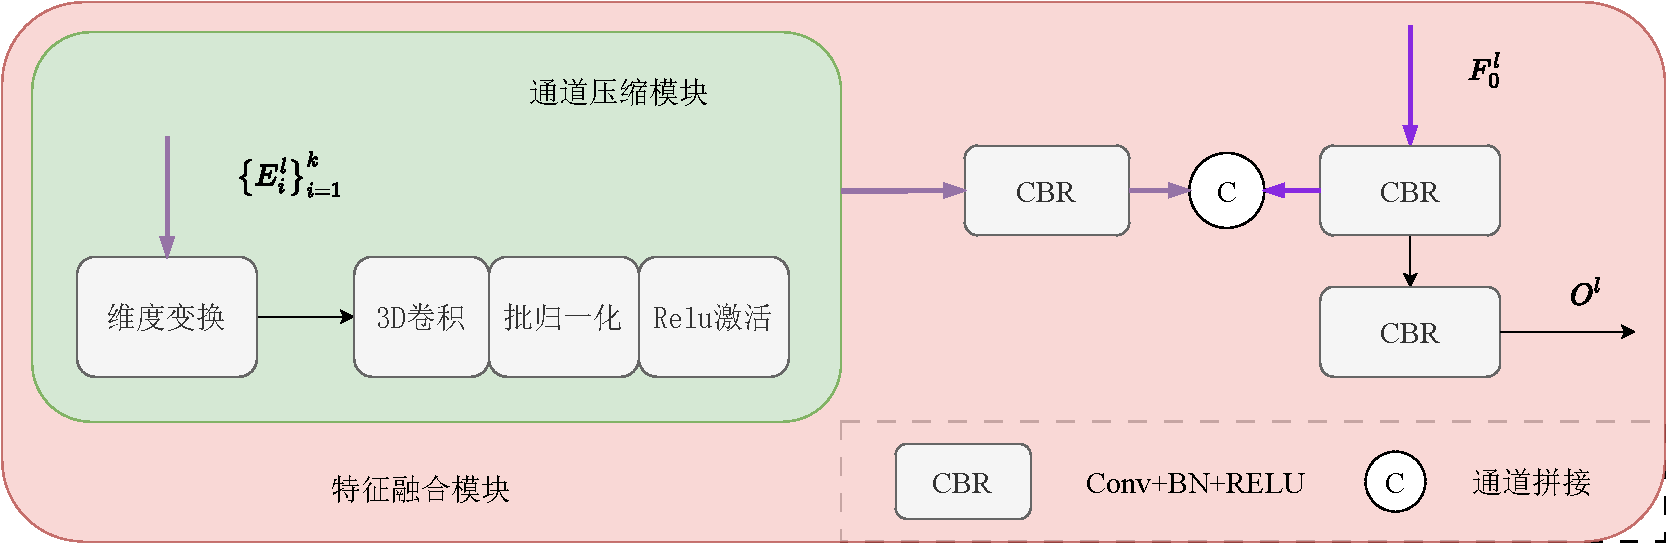
\includegraphics[width=0.95\linewidth]{figures/chapter3/ccm}
	\bicaption{
		特征融合模块。
	}{
		Feature fusion module.
	}  
	\label{cpt3_fig1:ccm}
\end{figure}
%
%
%
\par
%
%
我们提出了一种基于 3D 卷积的通道压缩模块 (Channel Compression Module,CCM) 来解决这个问题。 
通道压缩模块引入了3D卷积,它可以本质上提取时空特征来融合所有焦点堆栈特征。
具体来说,对于形状为 $ k \times C \times h \times w $ 的每一层增强焦点堆栈特征,
我们将其重塑为 $ C \times  k \times  h \times w $ ,然后使用内核为 $ k \times 1 \times 1 $  的 3D 卷积来融合空间上下文特征并压缩通道。 压缩特征 $ C^{l} $ 可以表示为:
%
%
%%
%%
\begin{equation}
	C^{l} = CCM \left ( Reshape \left ( E_{1-k}^{l} \right ) \right ) ,
\end{equation}
%%
%%
%
%
其中通道压缩模块主要由3D卷积组成,包括 $3DConv+BN+RELU$。 给定与输入形状相同的焦点堆栈和全焦点特征,采用多个卷积块进行跨域融合。 因此,我们将特征融合模块表述如下:
%
%
%	
%%
\begin{equation}
	%%
	O^{l}=CBR_{2}\left (Cat \left (CBR_{1} \left (F_{0}^{l} \right ),CBR_{1} \left (C^{l} \right ) \right ) \right ),
\end{equation}
%%
%%
%
%
其中 $CBR_{1}$ 和 $CBR_{2}$ 表示卷积块,包括 $Conv+BN+RELU$,前者使用 $1 \times C$ 通道输入,后者使用 $2 \times C$通道输入。
得到四层输出特征 $\left \{ O^{l} \right \}_{l=1}^{4} $ 后, 基于 FPN 的解码器~\cite{lin2017feature}~生成四个显着性预测图。 
其中最后一张用作最终的显着性预测图。 
%
%
%
%
%
%\BiSubsection{损失函数}{TODO}
\BiSubsection{训练过程}{TODO}
%
%
本文所提出的网络模型使用一个混合损失函数来训练。
%
%
二元交叉熵(Binary Cross Entropy,BCE)~\cite{de2005tutorial}~是二元分类和分割中使用最广泛的损失函数。 但 $\mathcal L_{bce} $ 是像素级损失,这意味着它平等对待所有像素。
在具有主导背景的图片中,前景像素的损失将会被稀释。 最近,显著性网络~\cite{qin2019basnet}~中引入了交并比(Intersection over Union,IoU)损失来弥补二元交叉熵损失的不足。
$ \mathcal L_{iou} $ 的目标是优化全局结构,而不是专注于单个像素,这样就不会受到分布不平衡的影响。 增强对齐度量~\cite{fan2018enhanced}~首先被提出作为一种可以同时考虑像素级和图像级误差的评估指标,
损失形式为 $ \mathcal L_{em} = 1 - E_{\xi} $。 

%
%
%
%
%
%
基于上述讨论,我们构建了一个混合损失:
%
%
%
%%
\begin{equation} 
	% L = L_{BCE} \left (  P,G \right )  + L_{IOU} \left ( P,G  \right ) + L_{EM} \left ( P,G  \right ) 
	\mathcal L = \mathcal L_{bce} + \mathcal L_{iou}  + \mathcal L_{em}  .
\end{equation}
%
%
%
%
\par
%
%
如图~\ref{cpt3_fig1:overview}~所示,我们的模型有两个掩码头,它们预测辅助显着性图 $ P^{A} $ 和四个最终多尺度显着性图 $ \left \{ P_{i}^{S} \right \}_{i=1}^{4} $ 。 因此,所提出的网络的总损失 $ \mathcal L_{total} $ 可以表示为: 
%
%% 
%%
%%
\begin{equation}
	\mathcal L_{total} = \mathcal L\left ( P^{A}, G \right ) + \lambda  \sum_{i=1}^{4} \left ( \mathcal L \left (  P_{i}^{S},G \right )\right ),
	%% \mathcal L_{total} = \mathcal L\left ( T_{0}, G \right ) + \lambda  \sum_{i=0}^{3} \left ( \mathcal L \left (  P_{i}^{S},G \right )\right )
	%% \mathcal L_{total} = \mathcal L\left ( T_{0}, G \right ) + \lambda  \sum_{i=0}^{3} \left ( \mathcal L \left (  P_{i},G \right )\right )
\end{equation}
%%
%%
%
%
%
其中 $ G $ 表示真值图。$ \mathcal L $代表我们用来逐渐优化预测的混合损失。 $ \lambda $是用于辅助控制监督项权重的超参数。
%
%
%
%
%
%
%
%
%
%
%
%

\BiSection{实验结果与分析}{TODO}

\BiSubsection{实验设置}{TODO}
%
%
%
%
%
(1)实验数据集
%
%
\par
%
%
我们的实验是在四个公共光场基准数据集上进行的:LFSD~\cite{li2014saliency}、HFUT~\cite{zhang2017saliency}、DUTLF-FS~\cite{zhang2019memory}~和 DUTLF-V2~\cite{piao2020dut}。 HFUT 和 LFSD 相对较小,分别仅包含 255 个和 100 个样本。 DUTLF-V2是最大的数据集,包含4204个样本,分为2957个和1247个分别用于训练和测试。 DUTLF-FS包含1462个样本,分别分为1000个训练样本和462个测试样本。 每个样本都包含一个全焦点图像、几个焦点切片以及相应的真值显着性图。
%
%
%
%
\par
%
%
%
%------------------------------ figure: comparison
\begin{figure*}
	\centering
	% \setlength{\abovecaptionskip}{-5mm}
	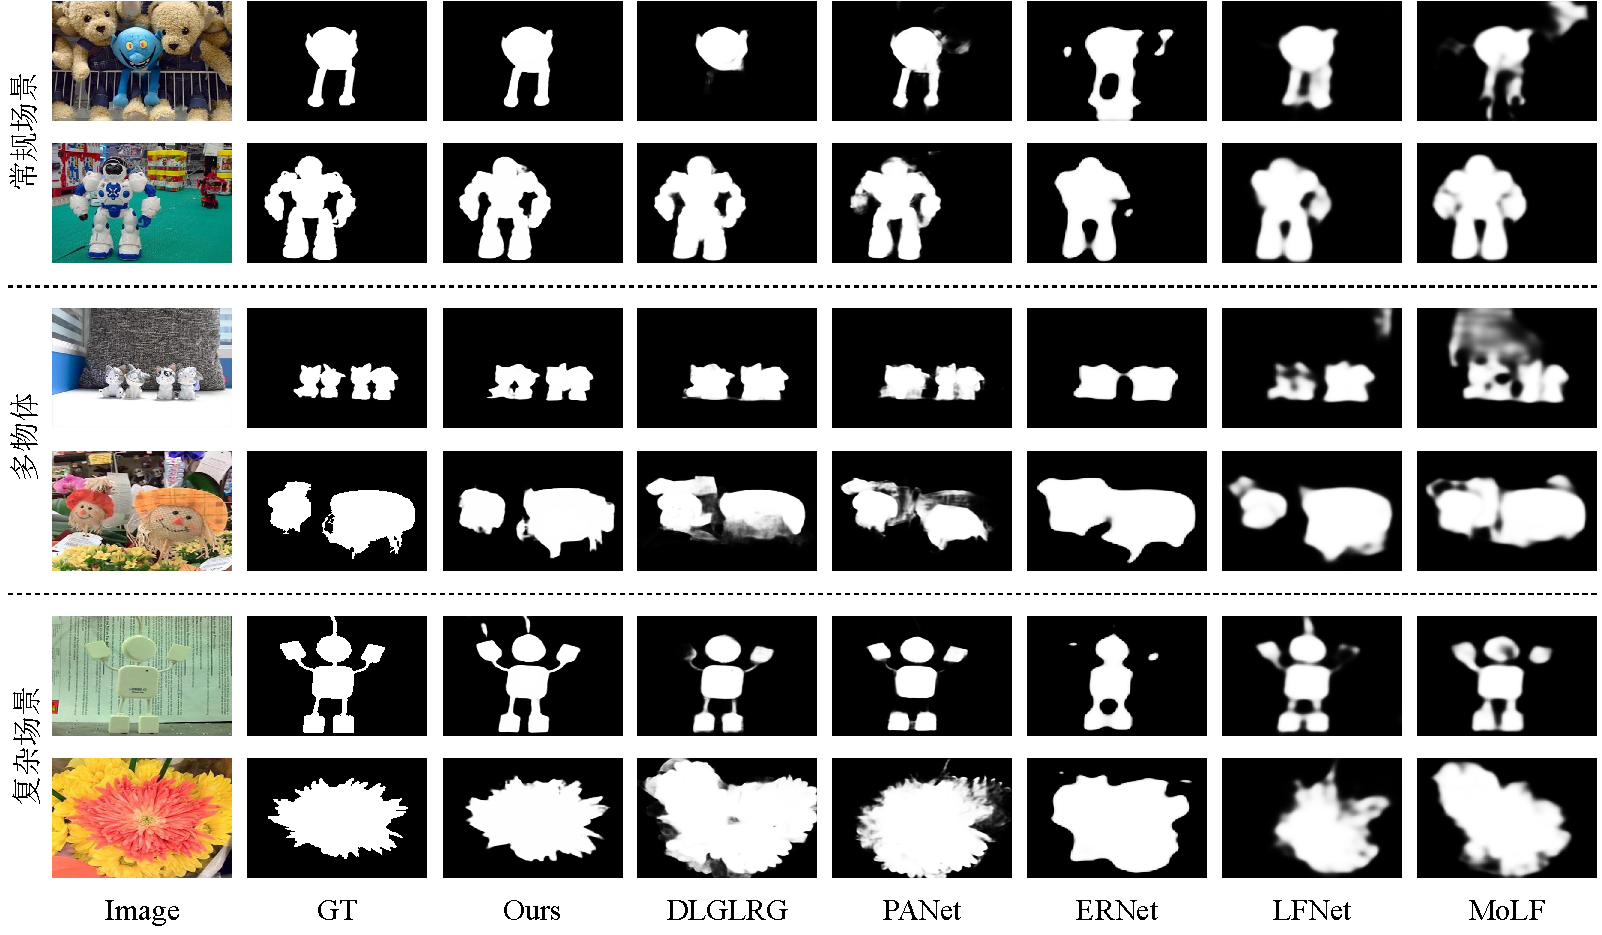
\includegraphics[width=\linewidth]{figures/chapter3/compare_1}
	\bicaption{
		在一些具有挑战性的场景(包括多物体和复杂场景)中对最先进的方法进行定性比较。
	}{
		Qualitative comparisons of state-of-the-art methods in some challenging scenes, including multiple objects and complex scenes.
	}
	\label{figure:figure_comparison_1}
	\vspace{-0.2cm}
\end{figure*}
%
%
%\\
%
(2)实现细节
%
%
\par
%
%
为了公平比较,我们遵循大多数以前的方法~\cite{piao2020exploit, liu2021light}~使用 DUTLF-FS 和 HFUT 的训练集来训练我们的 FPT,以便与使用焦点堆栈输入训练的其他光场方法进行比较。 我们按照~\cite{wang2022lfbcnet,jing2021occlusion}~使用 DUTLF-V2 的训练集来训练我们的模型,以便与使用多视图输入训练的其他最先进的 LFSOD 方法进行比较。 我们将每个图像的大小调整为 $256 \times 256$,以便于在训练和测试中实现,并且我们还通过随机翻转、裁剪和旋转来增强训练数据。
我们使用预训练的 PVT-B2~\cite{wang2022pvt}~模型作为我们的主干,因为它具有与 ResNet50~\cite{he2016deep}~相似的计算复杂性。 我们共享全焦点和焦点堆栈模式之间的主干权重,以减少不必要的参数。 整个网络使用 Adam~\cite{kingma2014adam}~作为优化算法进行端到端训练,并将初始学习率设置为 1e-4。 小批量大小设置为 2,我们的网络训练了 80 个循环迭代。 学习率在第 40 和 70 个迭代循环时分别乘以 0.1。 所提出的方法是使用Pytorch工具箱~\cite{paszke2017automatic}~实现的,所有实验都在四个RTX 1080Ti GPU上进行。 我们的代码将可用。 
%
%
%
%
%
\par
%
%
%\\
%\\
%
%
%
(3)评价指标
%
%
\par
%
%
本章采用了绝对平均误差、S-measure、E-measure和F-measure作为评
估模型性能的指标。





\BiSubsection{消融实验}{TODO}

定量比较:为了进行全面比较,我们将我们的方法与 26 个最先进的模型进行比较,
包括6个光场显著性分割方法:
DLGLRG \cite{liu2021light}, RENet \cite{piao2020exploit}, LFNet \cite{zhang2020lfnet},
MAC \cite{zhang2020light}, MoLF \cite{zhang2019memory}, and DLSD \cite{piao2019deep};
%
%
%
%
6个RGB-D显著性分割方法:
DCF \cite{ji2021calibrated}, CIR-Net \cite{cong2022cir}, VST-$rgbd$  \cite{liu2021visual},
BBS-Net     \cite{fan2020bbs}, SSF     \cite{zhang2020select} and S2MA    \cite{liu2020learning};
%
%
%
%
%
和14个2D显著性检测方法:
VST-$rgb$ \cite{liu2021visual},
PFSNet \cite{ma2021pyramidal},
ITSD \cite{zhou2020interactive},
LDF \cite{wei2020label},
MINet \cite{pang2020multi},
F$^{3}$Net  \cite{wei2020f3net}, 
EGNet   \cite{zhao2019egnet},
CPD  \cite{wu2019cascaded},
PoolNet \cite{liu2019simple},
PiCANet \cite{liu2018picanet},
PAGRN \cite{wang2018detect},
C2S   \cite{li2018contour},
R3Net  \cite{deng2018r3net}
和
Amulet \cite{zhang2017amulet}
。
%
%
%包括 7 个 LFSOD 方法:DLGLRG [21]、RENet [31]、LFNet [50]、MAC [47]、MoLF [51]和DLSD[30]; 6种RGB-D SOD方法:DCF [13]、CIR-Net [4]、VST-rgbd [20]、BBS-Net [10]、SSF [52]和S2MA [19]; 和 7RGB 方法:VST-rgb [20]、PFSNet [23]、ITSD [58]、LDF [44]、MINet [24]、F3 Net [43] 和 EGNet [56]。 
%
%
%
\par
%
%
为了保证公平比较,我们使用他们提供的显着性预测图或预训练的权重来生成比较数据,并利用~\cite{liu2021visual}~提供的相同评估代码。 
如表~\ref{table:comp_with_sota_3_1}~所示,
很明显,所提出的方法在 DUTLF-FS 和 HFUT 数据集上实现了比当前最先进的方法更优越的性能。 同时,所提出的方法可以在除了 $ S_{\alpha} $ 的另外三个指标上超越其他方法。 值得一提的是,与使用大量数据集训练的 RGBD 和 RGB 的显著性检测方法相比,我们的方法在小三倍的训练集(1100 vs. 2985 vs. 10553)下取得了显着的优势。 这表明我们的方法可以有效地探索光场数据中传达的信息。 
%
%
%
%
%
%
\begin{table*}[]
	%
	%---------------------------------------------------------------------> 大表 
	%
	%	\caption{Quantitative comparison of our proposed FPT with other 20 SOTA SOD methods on three benchmark datasets. 
		%		$ \uparrow \& \downarrow $ denote larger and smaller is better.
		%		%
		%		% denote the best and the second-best results,
		%		%
		%		The best three results are shown in 
		%		\textbf{boldface}, \textcolor{red}{red} and \textcolor{blue}{blue} fonts respectively. 
		%		% '-' indicates the code or outcome is not available.
		%	}
	\bicaption{
		在 3 个公开数据集上的定量比较
	}{Quantitative comparisons on three light field datasets}
	%	\renewcommand{\arraystretch}{1.5}
	
	\centering
	\label{table:comp_with_sota_3_1}
	%	\label{table:comp-with-sota}
	\resizebox{\textwidth}{!}{
		\begin{tabular}{rcccccccccccc}
			\toprule  %添加表格头部粗线
			
			% title
			%			\multirow{2}*{Type} & 
			\multicolumn{1}{c}{ \multirow{2}*{方法} } & 
			\multicolumn{4}{c}{DUTLF-FS \cite{zhang2019memory} } &
			\multicolumn{4}{c}{HFUT \cite{zhang2017saliency} } &
			\multicolumn{4}{c}{LFSD \cite{li2014saliency} } \\
			
			% next line
			\cmidrule(r){2-5} \cmidrule(r){6-9} \cmidrule(r){10-13}
			
			%			 subtitle
			& $E_{\phi}^{max}\uparrow$ & $S_{\alpha }\uparrow$ & $F_{\beta}^{max}\uparrow$ & MAE$\downarrow$ 
			& $E_{\phi}^{max}\uparrow$ & $S_{\alpha }\uparrow$ & $F_{\beta}^{max}\uparrow$ & MAE$\downarrow$  
			& $E_{\phi}^{max}\uparrow$ & $S_{\alpha }\uparrow$ & $F_{\beta}^{max}\uparrow$ & MAE$\downarrow$ \\
			
			%			& E & S & F & MAE 
			%			& E & S & F & MAE 
			%			& E & S & F & MAE \\
			
			
			% line line
			\midrule
			
			%			\multirow{8}*{\textit{Light field}}
			
			% 开始填数据
			
			Ours	 
			&  {\textbf{.973}} & \textbf{ {.946}} 	& \textbf{ {.954}} & \textbf{ {.020}} 
			& \textbf{ {.871}} &	\textbf{ {.828}} 			&\textbf{	 {.784}} & {\textcolor{red}{.064}} 
			& \textbf{ {.919}} &	\textcolor{blue}{.860} 			&	\textbf{ {.873}} &	\textbf{ {.064}} 
			\\
			
			DLGLRG \cite{liu2021light} 
			& {\textcolor{red}{.958}} & {\textcolor{red}{.928}} 			& {\textcolor{red}{.934}} & {\textcolor{red}{.029}} 
			&	.839 &	.766 &	.698 &	.070 
			&	{\textcolor{red}{.906}} &	\textbf{ {.866}} 			&	{\textcolor{red}{.870}} &	\textcolor{blue}{.069} 
			\\
			
			ERNet \cite{piao2020exploit}
			& .947 & .899 & .908 & .039 
			&	.841 &	.778 &	.722 &	.082 
			&	.888 &	.834 &	.850 &	.082 
			\\
			
			PANet \cite{piao2021panet} 
			& .939 & .908 & .903 & .038 
			& .845 & .795 & .738 & .074 
			& .892 & .849 & .849 & .076
			\\
			
			LFNet	 \cite{zhang2020lfnet} 
			& .929 & .878 & .890 & .053
			&	.846 &	.782 &	.718 &	.073 
			&	.885 &	.820 &	.824 &	.092 \\
			
			MAC	 \cite{zhang2020light} 
			& .863	& .804	& .792	& .102	
			&   .797 & .731 & .667 & .107 
			& .832 & .782 & .776 & .127 \\
			
			MoLF	 \cite{zhang2019memory} 
			& .938 & .887 & .902 & .051 
			&	.852 &	.789 &	.729 &	.075 
			&	.888 &	.830 &	.834 &	.089 \\
			
			DLSD	\cite{piao2019deep}
			& .891	& .841	& .801	& .076	
			&   .783 & .741 & .615 & .098 
			& .806 & .737 & .715 & .147 \\
			
			\midrule % end lfsod
			
			% start rgb-d
			%			\multirow{6}*{\textit{RGB-D}}
			
			DCF \cite{ji2021calibrated} 
			& \textcolor{blue}{.954} & \textcolor{blue}{.921} & \textcolor{blue}{.927} & \textcolor{blue}{.031} 
			& \textcolor{blue}{.856} & {\textcolor{red}{.812}} & {\textcolor{red}{.768}} & \textcolor{blue}{.065} 
			& .881 & .809 & .821 & .096 \\
			
			CIR-Net \cite{cong2022cir}
			& .950 & .916 & .921 & .038 
			& {\textcolor{red}{.862}} & .800  			& .742 & \textbf{ {.062}} 
			& .874 & .820 & .816 & .098 \\ 
			
			VST-$rgbd$  \cite{liu2021visual} 
			& .952 & .920 & .921 & .036 
			& .843 & .807 & .754 & .086 
			& .851 & .792 & .786 & .110 
			\\
			
			%			& -  & 2022  & \\
			%			& -  & 2022  & \\
			
			BBS-Net     \cite{fan2020bbs} 
			& .900 & .865 & .852 & .066 
			& .801 & .751 & .676 & .073 
			& \textcolor{blue}{.901} & {\textcolor{red}{.864}} & .858 & .072 \\ 
			
			SSF     \cite{zhang2020select} 
			& .922 & .879 & .887 & .050 
			& .816 & .725 & .647 & .090 
			& \textcolor{blue}{.901} & .859 & \textcolor{blue}{.868} & {\textcolor{red}{.067}} \\ 
			
			S2MA    \cite{liu2020learning} 
			& .839 & .787 & .754 & 	.102 
			& .777 & .729 & .650 & .112 
			& .873 & .837 &	.835 & .094 \\
			
			
			\midrule % end rgb-d
			%			\multirow{7}*{\textit{RGB}}
			
			VST-$rgb$ \cite{liu2021visual} 
			& .939 & .910 & .911 & .047
			& .831 & \textcolor{blue}{.808} & \textcolor{blue}{.763} & .093 
			& .865 & .797 & .817 & .123 
			\\ 
			
			PFSNet \cite{ma2021pyramidal}
			& .912 & .883 & .879 & .057 
			& .835 & .800 & .752 & .088 
			& .805 & .749 & .727 & .145 
			\\ 
			
			
			ITSD \cite{zhou2020interactive} 
			& .930 & .899 & .899 & .052 
			& .839 & .805 & .759 & .089 
			& .879 & .847 & .840 & .088 
			\\ 
			
			
			
			LDF \cite{wei2020label} 
			& .898 & .873 & .861 & .061 
			& .804 & .780 & .708 & .093 
			& .843 & .821 & .803 & .096 
			\\ 
			
			
			MINet \cite{pang2020multi} 
			& .916 & .890 & .882 & .050 
			& .816 & .792 & .720 & .086 
			& .861 & .834 & .828 & .091 
			\\ 
			
			F$^{3}$Net  \cite{wei2020f3net}
			& .900 & .888 & .882 & .057 
			& .815 & .777 & .718 & .095 
			& .824 & .806 & .797 & .106 
			\\ 
			
			
			EGNet   \cite{zhao2019egnet}
			& .914 & .886 & .870 & .053 
			& .794 & .772 & .672 & .094 
			& .776 & .784 & .762 & .118 
			\\ 
			
			CPD  \cite{wu2019cascaded}
			& .867 & .911 & .866 & .058 
			& .772 & .82  & .701 & .086 
			& .759 & .82  & .759 & .126 \\
			
			PoolNet \cite{liu2019simple}
			& .889 & .919 & .868 & .051 
			& .776 & .802 & .683 & .092 
			& .789 & .8   & .769 & .118 \\
			
			PiCANet \cite{liu2018picanet}
			& .829 & .892 & .821 & .083 
			& .726 & .781 & .618 & .115 
			& .729 & .78  & .671 & .158 \\
			
			PAGRN \cite{wang2018detect}
			& .822 & .878 & .828 & .084 
			& .717 & .773 & .635 & .114 
			& .727 & .805 & .725 & .147 \\
			
			C2S   \cite{li2018contour}
			& .844 & .874 & .791 & .084 
			& .763 & .786 & .65  & .111 
			& .806 & .82  & .749 & .113 \\
			
			R3Net  \cite{deng2018r3net}
			& .833 & .819 & .783 & .113 
			& .727 & .728 & .625 & .151 
			& .789 & .838 & .781 & .128 \\
			
			Amulet \cite{zhang2017amulet}
			& .847 & .882 & .805 & .030 
			& .767 & .76  & .636 & .110  
			& .773 & .821 & .757 & .135 \\
			
			
			\bottomrule % end
		\end{tabular}
	}
\end{table*}
%
%
%\\
%\\
%
\par
%
%
%
我们还在 DUTLF-V2 上重新训练我们的方法,并与其他三种使用多视图图像作为输入的 LFSOD 方法进行比较,包括 OBGNet ~\cite{jing2021occlusion}、LFBCNet~\cite{wang2022lfbcnet}~ 和 ESCNet~\cite{zhang2022exploring}。 如表~\ref{table:comp_multi_view}~所示,我们的方法可以在 DUTLF-V2 的所有四个指标上大幅实现最佳性能。 这证明了使用焦点堆栈作为输入的优越性。 
%
%
%
%---------------------------------------------------------------------> 消融实验: 多视角方法对比
%
\begin{table}
	%	\caption{Quantitative results of comparison with multi-view LFSOD methods.
		%		- means unavailable results.
		%		The best results are marked in \textbf{boldface}.
		%		% \textbf{Bold} indicates the best performance.
		%		% The best results are marked in boldface.
		%	}
	\bicaption{	与多视图 LFSOD 方法比较的定量结果。}{
		Quantitative results of comparison with multi-view LFSOD methods.
	}
	\centering
	\label{table:comp_multi_view}
	%	\resizebox{\linewidth}{!}{
		\begin{tabular}{crcccc}
			\toprule  %添加表格头部粗线
			
			% title
			\multirow{2}*{Input Types} & \multicolumn{1}{c}{\multirow{2}*{Methods}} & \multicolumn{4}{c}{DUTLF-V2 \cite{piao2020dut}} \\
			
			% next line
			\cmidrule(r){3-6} 
			
			% subtitle
			& & $E_{\phi}^{max}\uparrow$ & $S_{\alpha }\uparrow$ & $F_{\beta}^{max}\uparrow$ & MAE$\downarrow$ \\
			
			\midrule  % E S F MAE
			
			Focal stack       & \multicolumn{1}{c}{ Ours$^{\ast} $ } &
			\textbf{ 0.960 } & \textbf{ 0.923 }  & \textbf{ 0.917 }  & \textbf{ 0.026 }  \\ 
			%								 &  0.9598 & 0.9227 & 0.9173 & 0.0256 \\
			% multiview
			
			\midrule
			\multirow{3}*{Multi-view}
			& OBGNet \cite{jing2021occlusion}      &  0.940  & 0.896  & 0.885  & 0.037  \\
			& LFBCNet \cite{wang2022lfbcnet}    &  0.940  & 0.890  & 0.870  & -      \\
			& ESCNet \cite{zhang2022exploring}      &  0.931  & 0.882  & 0.852  & 0.041  \\
			
			
			\bottomrule
		\end{tabular}
		%}
\end{table}
%
%
\par
%
%
定性比较:为了更直观地观察,
图~\ref{figure:figure_comparison_1}~
\ref{figure:figure_comparison_2}~
\ref{figure:figure_comparison_3}~
中可视化了所提出的方法和其他排名靠前的方法生成的一些代表性结果。可以看出,我们提出的方法的结果与真值图更加一致。 当面对这些具有挑战性的场景时,包括多个对象(第 4、5 行)和复杂场景(第 6、7 行),大多数 RGB 和 RGB-D 显著性检测方法无法准确检测显着对象。
相比之下,我们所提出的方法可以成功生成准确且稳健的显着图。 与这些基于 CNN 的 LFSOD 方法相比,所提出的方法获得了更一致的预测结果和更精细的细节。
%
%
%
%
%
%
%
%
%



	%------------------------------ figure: comparison
\begin{figure*}
	\centering
	% \setlength{\abovecaptionskip}{-5mm}
	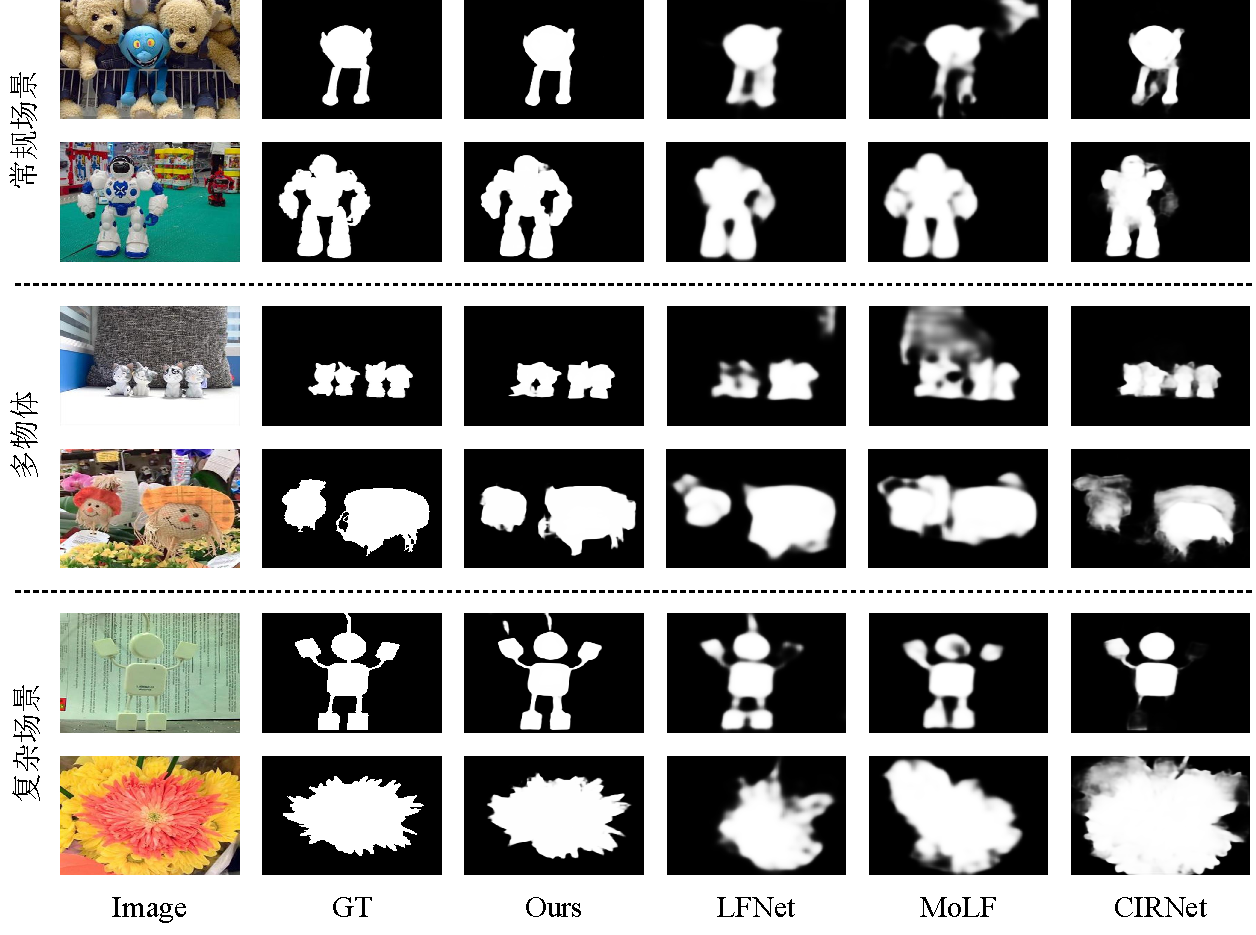
\includegraphics[width=\linewidth]{figures/chapter3/compare_2}
%	\caption{
%		Qualitative comparisons of state-of-the-art methods in some challenging scenes, including multiple objects and complex scenes.
%	}
	\bicaption{
		在一些具有挑战性的场景(包括多物体和复杂场景)中对最先进的方法进行定性比较。
	}{
		Qualitative comparisons of state-of-the-art methods in some challenging scenes, including multiple objects and complex scenes.
	}
	\label{figure:figure_comparison_2}
	\vspace{-0.2cm}
\end{figure*}

	%------------------------------ figure: comparison
\begin{figure*}
	\centering
	% \setlength{\abovecaptionskip}{-5mm}
	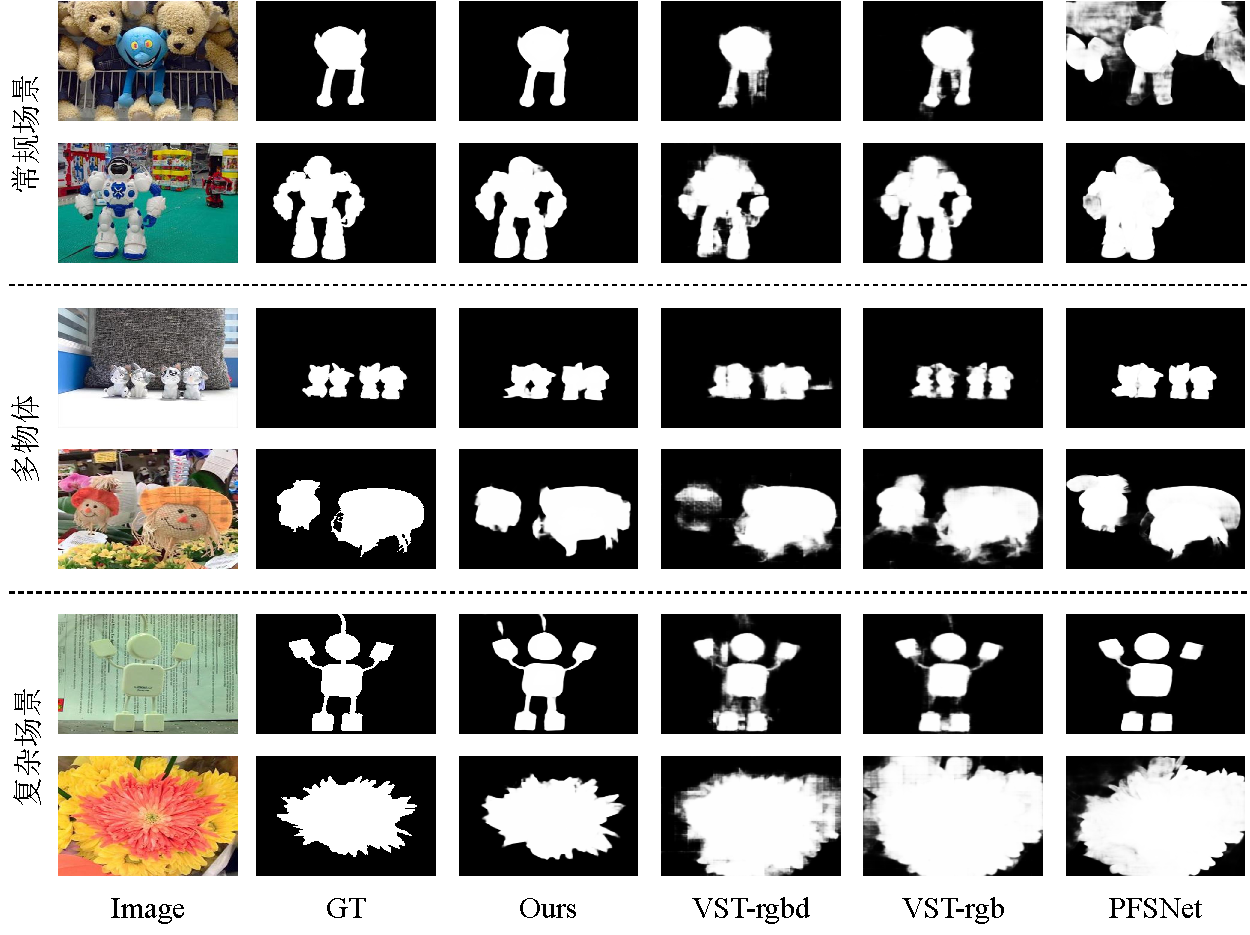
\includegraphics[width=\linewidth]{figures/chapter3/compare_3}
%	\caption{
%		Qualitative comparisons of state-of-the-art methods in some challenging scenes, including multiple objects and complex scenes.
%	}
	\bicaption{
		在一些具有挑战性的场景(包括多物体和复杂场景)中对最先进的方法进行定性比较。
	}{
		Qualitative comparisons of state-of-the-art methods in some challenging scenes, including multiple objects and complex scenes.
	}
	\label{figure:figure_comparison_3}
	\vspace{-0.2cm}
\end{figure*}
% 
%
%
%\\
%\\% 
%---------------------------------------------------------------------> 消融实验: 总消融实验
%
\begin{table}
%	\caption{Ablation analyses of each component on the DUTLF-FS dataset.
%		The best results are marked in \textbf{boldface}.
%	}
	\bicaption{
	DUTLF-FS 数据集上每个组件的消融分析。
	}{
	Ablation analyses of each component on the DUTLF-FS dataset.
	}
	\centering
	\label{table:abl_total}
%	\resizebox{0.82\linewidth}{!}{
		\begin{tabular}{llcccc}
			\toprule  %添加表格头部粗线
			%%  \multicolumn{1}{c}{ \multirow{2}*{Methods} }
			
			\multicolumn{2}{c}{ \multirow{2}*{Settings}}	& \multicolumn{4}{c}{DUTLF-FS} \\ %& \multicolumn{3}{c}{HFUT} \\ 
			
			\cmidrule(r){3-6} 
			
			& & $E_{\phi}^{max}\uparrow$ & $S_{\alpha }\uparrow $ & $F_{\beta}^{max}\uparrow$ & MAE$\downarrow$ \\
			\midrule
			
			% 开始填写数据
			\multicolumn{2}{l}{ Baseline }     & 0.947 & 0.894 & 0.901 & 0.048 \\ 
			
			%		 			\multicolumn{2}{l}{+Token} 	 & 0.959 & 0.918 & 0.926 & 0.037 \\ 
			
			\midrule
			
			\multicolumn{1}{c}{ \multirow{2}*{+TCM}}	
			
			& +TI		& 0.961 & 0.923 & 0.932 & 0.034 \\ 
			& ++TS & 0.968 & 0.933 & 0.944 & 0.027 \\
			\midrule
			
			\multicolumn{2}{l}{++FPE} 		& \textbf{0.972} & 0.941 & 0.952 & 0.022 \\
			\multicolumn{2}{l}{+++CCM} 		& \textbf{0.972} & \textbf{0.942} & \textbf{0.953} & \textbf{0.021} \\ 
			
			
			\bottomrule
	\end{tabular}
% }
\end{table}

%---------------------------------------------------------------------> figure: overview 
\begin{figure}[t] 
	% \centering
	%	\begin{center}
		%	\includegraphics[width=0.95\linewidth]{figures/overview.pdf} 		
		%	\end{center}
	
	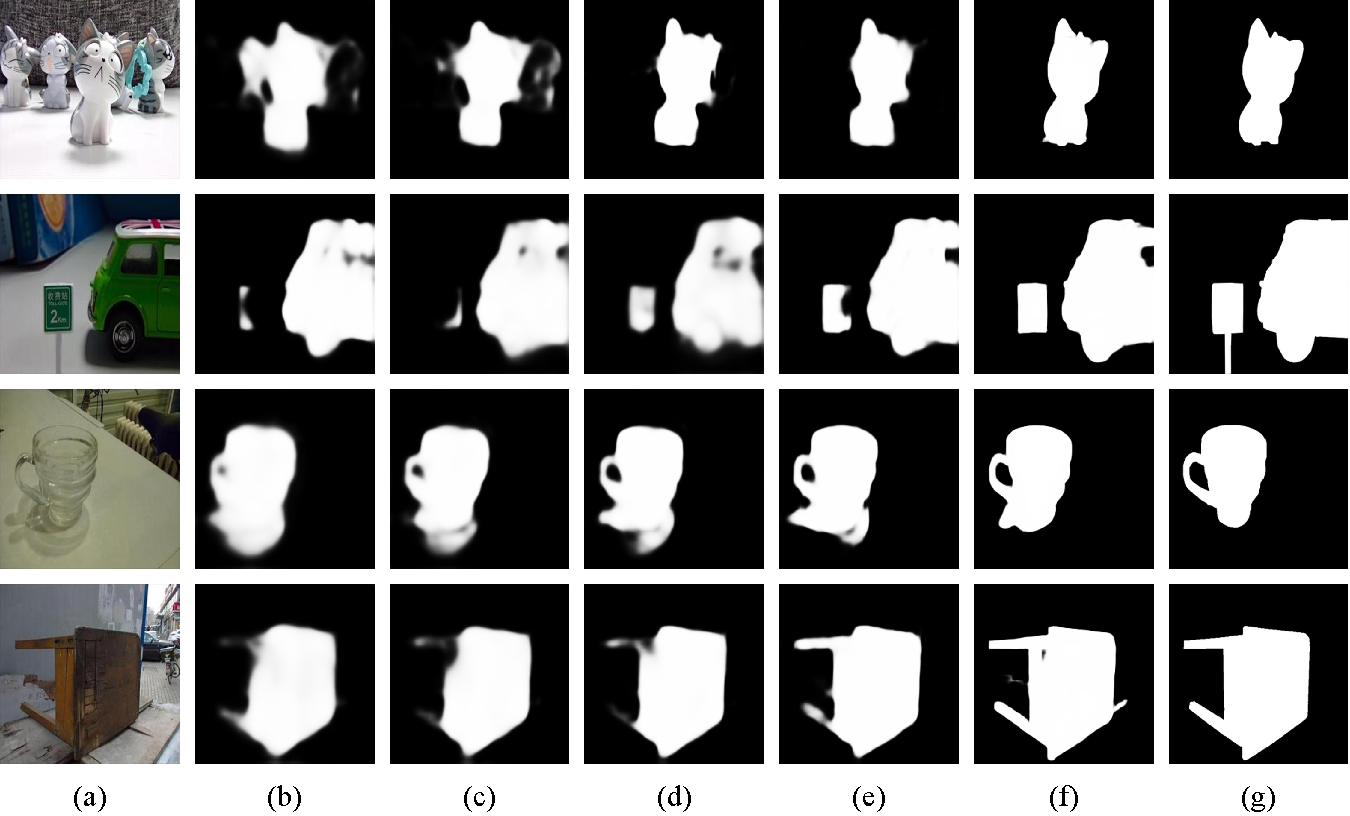
\includegraphics[width=0.99\linewidth]{figures/chapter3/self-comparsion-Use} 
	\centering
	
	
%	\caption{   	Visual comparisons of ablation studies.      (a) All-focal images.      
%		(b)-(f) Saliency maps of the ``Baseline'', ``+TCM (+TI)'', ``+TCM (++TS)'', ``++FPE'' and ``+++CCM'', respectively.
%		%			
%		%			(b) Saliency maps of baseline.
%		%			(c) Saliency maps w TCM (w/o TS).
%		%			(d) Saliency maps w TCM.
%		%			(e) Saliency maps w using FPE.
%		%			(f) Saliency maps w using CCM.
%		(g) Ground truth maps.
%	}  
%	
	\bicaption{
	消融研究的可视化比较。 
%	(a) 全聚焦图像,
%	(b)-(f) 分别为“基线模型”、
%	“+TCM (+TI)”、
%	“+TCM (++TS)”、
%	“++FPE”和
%	“+++CCM图”的显著性图。
	}{
	Visual comparisons of ablation studies.      
%	(a) All-focal images.      
%	(b)-(f) 
%	Saliency maps of the ``Baseline'', 
%	``+TCM (+TI)'', 
%	``+TCM (++TS)'', 
%	``++FPE'' and 
%	``+++CCM'', respectively.
%	(g) Ground truth maps.
	}
	\label{figure:self_comp}
	
	\vspace{-0.2cm}
\end{figure}



\BiSubsection{对比实验}{TODO}

\textbf{不同模型组件的有效性。}
我们首先在表~\ref{table:abl_total}~中验证不同模型组件的有效性。我们首先构建一个基线模型。 具体来说,它使用共享权重编码器来提取全焦点和焦点堆栈特征,然后直接连接它们并预测显着性图。 
%
%
%
%
\par
%
%
%
接下来,我们逐渐将我们提出的 TCM、FPE 和 CCM 采用到我们的 FPT 模型中。 这三个模型分别表示为“+TCM”、“++FPE”和“+++CCM”。 
如表~\ref{table:abl_total}~所示,这三个模型可以逐渐提高LFSOD性能,最终大幅优于基线模型。 
%
%
%
%
\par
%
%
%
此外,为了证明我们TCM中TI和TS子模块的有效性,我们逐渐在“+TCM”模型中采用TI和TS,并将它们表示为“+TI”和“++TS”。 与“基线”相比。 “+TI”和“++TS”在 DUTLF-FS 上分别使 MAE 指标降低 29.2\% 和 43.8\%。 
%
%
%
%
%
%
\par
%
%
%
%
%
%
%
我们还在图~\ref{figure:self_comp}~中提供了每个消融研究相应的可视化结果,
其中(a)表示全聚焦图像,
	(b)-(f) 分别代表“基线模型”、
	“+TCM (+TI)”、
	“+TCM (++TS)”、
	“++FPE”和
	“+++CCM”的显著性图。
可以发现,预测掩模与真值图逐渐变得更加一致。 显着对象的完整内容和精确的显着图边界证明我们的 F焦点感知Transformer模型可以过滤掉背景干扰并更多地关注显着对象。 
%
%
%
%
%
\par
%
%
%
\textbf{焦点相关标记的数量。} 
在表~\ref{table:abl_token_number}~中,我们用焦点相关标记的数量从 8 个增加到 32 个来测试我们的方法。与较少的焦点相关标记 (M = 8, 16) 相比,更多的焦点相关标记 (M = 32) 可以获得更好的结果 。 除非另有说明,我们的实验均使用 32 个与焦点相关的标记进行。 
%
%\\
%
%
%
%
\par
%
%
\textbf{焦点感知增强中的 $K$ 值。 }
我们设置了多个比较实验来选择最佳 $k$ 数,具体数据见表~\ref{table:abl_fp}。
当我们将 $K$ 从 1 增加到 5 时,性能逐渐提高。 当 $K > 5$ 时,我们观察到模型性能饱和并变得次优。 我们认为较大的 $K$ 值会引入更多不显着的背景效应。 考虑到性能和计算成本之间的权衡,我们选择配置 $K = 5$ 作为最终配置。

%---------------------------------------------------------------------> 消融实验: 焦点感知实验
%
\begin{table}
%	\caption{Impact of focal-related token numbers. $M $ indicates the number of focal-related tokens. 
%		%
%		%			Comparison of using different K numbers in focal perception enhancement strategy.
%		The best results are marked in \textbf{boldface}.
%	}
	\bicaption{
	焦点相关令牌数量的影响。 $M$表示焦点相关令牌的数量。}{
	Impact of focal-related token numbers. $M $ indicates the number of focal-related tokens. 
	}
	\centering
	\label{table:abl_token_number}
%	\resizebox{0.68\linewidth}{!}{
		\begin{tabular}{ccccc}
			\toprule  %添加表格头部粗线
			
			% title
			\multirow{2}*{$M$} & \multicolumn{4}{c}{DUTLF-FS} \\ % & \multicolumn{3}{c}{HFUT} \\
			
			% next line
			\cmidrule(r){2-5} % \cmidrule(r){5-7} % \cmidrule(r){7-8} 
			
			% subtitle
			& $E_{\phi}^{max}\uparrow$ & $S_{\alpha }\uparrow $ & $F_{\beta}^{max}\uparrow$ & MAE$\downarrow$\\
			% & $S_{\alpha }\uparrow $ & $F_{\beta}^{max}\uparrow$ & MAE$\downarrow$ \\
			
			\midrule
			
			% 开始填写数据
			%% 8 & 0.969 & 0.934 & 0.944 & 0.026 \\ 
			
			8 &  0.967 & 0.936 & 0.946 & 0.025 \\ 
			16 & 0.970 & 0.937 & 0.948 & 0.024 \\
			32 & \textbf{0.972} & \textbf{0.941} & \textbf{0.952} & \textbf{0.022} \\ 
			
			\bottomrule
		\end{tabular}
%	}
	
	\vspace{-0.2cm}
\end{table}


% 
%---------------------------------------------------------------------> 消融实验: 焦点感知实验
%
\begin{table}
%	\caption{Comparison of using different K numbers in focal perception enhancement strategy.
%		The best results are marked in \textbf{boldface}.
%	}
	\bicaption
	{
		焦点感知增强策略中使用的不同K数的比较。
	}
	{
		Comparison of using different K numbers in focal perception enhancement strategy.
	}
	\centering
	\label{table:abl_fp}
%	\resizebox{0.68\linewidth}{!}{
		\begin{tabular}{ccccc}
			\toprule  %添加表格头部粗线
			
			% title
			\multirow{2}*{K} & \multicolumn{4}{c}{DUTLF-FS} \\ % & \multicolumn{3}{c}{HFUT} \\
			
			% next line
			\cmidrule(r){2-5} % \cmidrule(r){5-7} % \cmidrule(r){7-8} 
			
			% subtitle
			& $E_{\phi}^{max}\uparrow$ & $S_{\alpha }\uparrow $ & $F_{\beta}^{max}\uparrow$ & MAE$\downarrow$\\
			% & $S_{\alpha }\uparrow $ & $F_{\beta}^{max}\uparrow$ & MAE$\downarrow$ \\
			
			\midrule
			
			% 开始填写数据
			1 & 0.969 & 0.934 & 0.944 & 0.026 \\ 
			3 & 0.969 & 0.937 & 0.947 & 0.024 \\ 
			5 & \textbf{0.972} & \textbf{0.941} & \textbf{0.952} & \textbf{0.022} \\ 
			7 & 0.971 & 0.940 & 0.951 & \textbf{0.022} \\ 
			9 & 0.971 & 0.938 & 0.951 & 0.023 \\ 
			
			\bottomrule
		\end{tabular}
%	}
	\vspace{-0.2cm}
\end{table}




\begin{table}
%	\caption{Ablation results of different methods for focal perception enhancement module.
%		The best results are marked in \textbf{boldface}.
%	}
	\bicaption{
	焦点感知增强模块中不同方法的消融结果。}{
	Ablation results of different methods for focal perception enhancement module.
	}
	\centering
	\label{table:abl_methods}
%	\resizebox{0.45\linewidth}{!}{
		\begin{tabular}{ccccc}
			\toprule  %添加表格头部粗线
			
			% title
			\multirow{2}*{Settings} & \multicolumn{4}{c}{DUTLF-FS} \\  % & \multicolumn{3}{c}{HFUT} \\
			
			% next line
			\cmidrule(r){2-5} % \cmidrule(r){5-7} % \cmidrule(r){7-8} 
			
			% subtitle
			& $E_{\phi}^{max}\uparrow$ & $S_{\alpha }\uparrow $ & $F_{\beta}^{max}\uparrow$ & MAE$\downarrow$ \\
			% & $S_{\alpha }\uparrow $ & $F_{\beta}^{max}\uparrow$ & MAE$\downarrow$ \\
			
			\midrule
			
			% 开始填写数据
			Random      & 0.962 & 0.924 & 0.932 & 0.033 \\ 
			Conv        & 0.967 & 0.931 & 0.942 & 0.027 \\ 
			SSIM        & \textbf{0.972} & \textbf{0.941} & \textbf{0.952} & \textbf{0.022} \\ 
			%% Log(SSIM)   & \textbf{0.972} & 0.940 & 0.950 & 0.023 \\ 
			
			\bottomrule
	\end{tabular}
	\vspace{-0.2cm}
\end{table}


\textbf{焦点感知增强方法设置。}
为了验证不同焦点感知增强设置的有效性,我们在随机、卷积和基于 SSIM 的选择方法之间进行了比较实验。 所有实验将 $K$ 数设置为 5。表~\ref{table:abl_methods}~表明我们使用基于卷积方式进行感知增强的方法已经达到了与其他 LFSOD 方法相当的性能,证明了我们提出的方法的优越性。


\BiSection{本章小结}{TODO}

在本文中,我们提出了一种用于精确光场显着物体检测的焦点感知Transformer(FPT)。 我们引入与焦点相关的令牌来收集图像特定的特征,并提出令牌通信模块(TCM)来传播信息并促进空间上下文建模。 为了增强焦点堆栈的空间特征表示,我们提出了一种焦点感知增强(FPE)策略来帮助抑制噪声背景信息。 实验结果表明,我们提出的方法可以在大多数光场显著性分割数据集上实现最先进的性能。